\documentclass[12pt, oneside]{article}   	% use "amsart" instead of "article" for AMSLaTeX format
%\documentclass[12pt, oneside, draft]{article}   	% use "amsart" instead of "article" for AMSLaTeX format

%%%%%%%%%%%%%%%%%%%%%%%%%%%%%%%%%%%%%%%%%%%%%%%%%
%
% The TexLive distribution is stored in /usr/local/texlive/2020
%
% The definitions of the packages are in /usr/local/texlive/2020/texmf-dist/tex/latex
%
%%%%%%%%%%%%%%%%%%%%%%%%%%%%%%%%%%%%%%%%%%%%%%%%%

\usepackage{xparse}					% Allows for the creation of \NewDocumentCommand shortcuts

\usepackage{geometry}				% See geometry.pdf to learn the layout options. There are lots.
\geometry{letterpaper}				% ... or a4paper or a5paper or ... 
\usepackage[parfill]{parskip}		% Activate to begin paragraphs with an empty line rather than indent
\usepackage{graphicx}				% Use pdf, png, jpg, or eps§ with pdflatex; use eps in DVI mode
									% TeX will automatically convert eps --> pdf in pdflatex
\usepackage{float}					% Float package to exert more control over graphic placement
	
%\usepackage{verbatim}				% Creates a verbatim environment for code / program output

% Math packages
\usepackage{amssymb}				% Mathematical symbols
\usepackage{amsmath}				% Added for typesetting mathematical formulae
\usepackage{amsthm}					% Added for typesetting mathematical theorems
\usepackage{mathalpha}				% Added for some special characters like Q, Z and N

% Table packages in addition to built in tabular
\usepackage{booktabs}				% Adds extra commands to tabular like \toprule
\usepackage{afterpage}				% For pagination support
\usepackage{longtable}				% Support for longer tables

% Hyperlinks
\usepackage{hyperref}				% For creating internal and HTTP links

% For Tikz graphics
\usepackage{tikz}					% Package for pgf and TikZ
\usetikzlibrary{shapes,arrows,chains}
\tikzstyle{startstop} = [very thick, rectangle, rounded corners, minimum width=2.5cm, minimum height=0.8cm, text centered, draw=black, text width=2.5cm]
\tikzstyle{action} = [rectangle, rounded corners, minimum width=3cm, minimum height=0.8cm, text centered, draw=black, text width=2.5cm]
\tikzstyle{decision} = [diamond, minimum width=3cm, minimum height=3cm, text centered, draw=black, text width=2cm]
\tikzstyle{arrow} = [thick,->,>=stealth]

% For theorems and definitions - each creates it's own counter which incrementa each use
\theoremstyle{definition}
\newtheorem{proposition}{Proposition}[section]
\newtheorem{define}{Definition}[section]
\newtheorem{axiom}{Axiom}[section]
\newtheorem{theorem}{Theorem}
\newtheorem{lemma}[theorem]{Lemma}
\newtheorem{corollary}[theorem]{Corollary}

%SetFonts


\title{Collatz Conjecture Anti-Cyclicity}
\author{Wayne Brassem}
%\date{}							% Activate to display a given date or no date


\begin{document}

% Document define commands for commonly used items in math mode
\NewDocumentCommand{\setN}{}{\mathbb{N}}				% Set of positive integers, excluding 0
\NewDocumentCommand{\setNo}{}{\mathbb{N}_0}				% Set of positive integers, including 0
\NewDocumentCommand{\setNeven}{}{\mathbb{N}_{even}}		% Set of even positive integers, excluding 0
\NewDocumentCommand{\setNodd}{}{\mathbb{N}_{odd}}		% Set of odd positive integers
\NewDocumentCommand{\setZ}{}{\mathbb{Z}}				% Set of all integers, excluding zero
\NewDocumentCommand{\setZo}{}{\mathbb{Z}_0}				% Set of all integers, including zero
\NewDocumentCommand{\setQ}{}{\mathbb{Q}}				% Set of all rational numbers

% Document define commands for commonly used items not in math mode
\NewDocumentCommand{\Rarr}{}{\textrightarrow{}}			% Right arrow

% Document commands which provide hyperlinks to OEIS sequences referenced herein
\NewDocumentCommand{\OEIS}{m}{\href{https://oeis.org/#1}{#1}}

\maketitle



\begin{abstract}

%Abstract - goals of the paper
This aim of this paper is to establish that cycles (exclusive of 4\Rarr2\Rarr1\Rarr4) cannot exist within the positive integer space when positive integers are subjected to the odd number $\frac{3x+1}{2}, x \in \setN$ expansion and the recursive divide even numbers by 2 as per the Collatz Conjecture mapping $f: \setN$\Rarr $\setN$:

\[
f(x) = \begin{cases}
\displaystyle
    \phantom{3x} \frac{x}{2} & \text {if } x \text{ is even}, \\[8pt]  % Insert some spacing between rows
\displaystyle
    \frac{3x+1}{2}           & \text {if } x \text{ is odd}. \\
\end{cases}
\]


The process begins by utilizing the fact that the dropping pattern of residue classes generates the cardinality of convergent subsequences of a given length, where each convergent subsequence is associated with a non-overlapping subset of the positive integer space.  It is shown that associative groupings of residue equivalence class fractions of the positive integer space grows equal to or greater than terms from another well defined sequence.  This other sequence is known to converge to unity in the limit - squeezing the cumulative sum of residue groupings to unity as the residue path length goes to infinity.

When the cumulative summation of associative groupings of convergent fractional subsets goes to unity as the path length goes to infinity, it follows that every element of every residue class flows over a convergent subsequence, which means that each positive integer member element eventually converges to a smaller positive integer upon completion of the subsequence.

The fact that all positive integers eventually reach a smaller magnitude eliminates the possibility of a positive integer cycle.  More importantly, it means that by chaining together a series of convergent equivalence class subsequences, the complete orbit will ultimately reach the terminating 4\Rarr2\Rarr1\Rarr4 cycle, passing through 1 \emph{before} cycling back to 4 in complete agreement with the Collatz Conjecture.

\end{abstract}
\newpage


\tableofcontents
\newpage



\section{Introduction and Structure of Proof}
This paper shows how to construct a series, which grows to encompass the entire positive integer space, composed of convergent residue classes of positive integers such that all elements belonging to each of these classes converge to a smaller value over a finite subsequence.  Each convergent residue class represents a non-overlapping subset of the positive integers where \emph{all} elements converge to smaller positive integers over the subsequence whose length depends on the specific residue class.

The number of convergent residue classes for a given subsequence length is defined by the Online Encyclopedia of Integer Sequences (OEIS) sequence \OEIS{A186009} \cite{OEIS_A186009}.  The non-linear sequence \OEIS{A186009} is compared with a lesser integer sequence \OEIS{A047749} \cite{OEIS_A047749} whose integer term values are defined by an expression utilizing Gamma functions.  The logarithmic convexity of the  functional representation of \OEIS{A047749} is shown using the second PolyGamma derivative which remains greater than zero (convex up) for all positive values.  This fact establishes the logarithmic convexity of both of the series since \OEIS{A186009} is greater than or equal to \OEIS{A047749} on a term by term basis.

An associative grouping, without changing the order, of convergent subsets of positive integers is constructed so that every grouping is $\ge \frac{1}{2^k};k \in \setNo$ for all $k$.  The number of non-overlapping subsets in each grouping is shown to be less than or equal to the Pascal's triangle $k-2$ diagonal. As the number of groupings goes to infinity, the cumulative total of convergent groupings is squeezed by the well known identity
\[    \label{sum_infinite_halves}
    \lim_{n \to \infty} \sum_{k=1}^n { \frac{1}{ 2^k} } = 1
\]
which converges to unity in the limit.  Thus, all positive integers are members of some convergent equivalence class which are then guaranteed to converge to smaller integers as the subsequence length goes to infinity in the limit.

The orbit defines the path that any given positive integer takes using the aformentioned $f: \setN$\Rarr $\setN$ Collatz Conjecture mapping, which could in principle produce a cyclical loop.  However, if it can be shown that all finite integers converge to a smaller value, cycles in the positive integer space become impossible other than the obvious (and perfectly acceptable) exception of the terminating cycle 4\Rarr2\Rarr1\Rarr4 which in no way stands in violation of the Collatz Conjecture.

Then, by chaining together a sufficient number of convergent orbit subsequences, one arrives at the inescapable conclusion that starting with any positive integer the complete orbit always converges to 1.



\newpage

\section{Conjecture Definitions}

The Collatz Conjecture states that for every positive integer ($x \in \setN$) there exists an iterative mapping $f: \setN$\Rarr $\setN$ with total stopping time $t$ so that $f^t(x)=1$, where:

\begin{equation}
\label{Collatz}
f(x) = \begin{cases}
\displaystyle
    \phantom{3x} \frac{x}{2} & \text {if } x \text{ is even}, \\[8pt]  % Insert some spacing between rows
\displaystyle
    \frac{3x+1}{2}           & \text {if } x \text{ is odd}. \\
\end{cases}
\end{equation}

We also define the stopping time, $\sigma(x)$, as a mapping $f: \setN$\Rarr $\setN$ where:

\begin{equation}
\label{sigma}
	\sigma(x) = k \text{ for } f^k(x)<x \text{ such that } k \text{ is minimal.}
\end{equation}


Throughout this paper, the following terms are used, therefore formal definitions of what is meant is provided.

\begin{define}
The \emph{stopping time} is the smallest $k$ of $f^k(x)$ such that $f^k(x) < x$.  In other words $k$ represents the smallest number of iterations of $f(x)$ which maps to a positive integer with a smaller magnitude than $x$, represented by $\sigma(x)$ as per (\ref{sigma}).
\end{define}

\begin{define}
A \emph{subsequence} is a path which follows the odd number $\frac{3x+1}{2}$ expansion and the recursive divide even numbers by 2 per (\ref{Collatz}).  The subsequence length is less than or equal to the length of the complete orbit which begins with the starting integer and concludes at the repeating terminating cycle 4\Rarr2\Rarr1\Rarr4.
\end{define}

\begin{define}
An \emph{equivalence class} is an infinite subset of the positive integer space having a characteristic equation $x \equiv y$ (mod $2^k$) allowing all members of the class to be found that are congruent to $y$.  It is therefore a fraction between 0 and 1 of the complete set of positive integers.
\end{define}

\begin{define}
A \emph{convergent subsequence} is the subsequence of minimum length, $k$, which when followed for all positive integers belonging to a given equivalence class will reach other positive integers with smaller magnitudes.  The length of this subsequence thus defines the stopping time, $\sigma(x)=k$.
\end{define}

\begin{define}
A \emph{residue class} is an convergent equivalence class represented by a non-overlapping infinite subset of the positive integer space which is associated with a convergent subsequence and thus has a finite stopping time.  Therefore, once the convergent subsequence path of length $\sigma(x)=k$ has been followed \emph{all} members of the residue class will have reached a smaller integer.
\end{define}

\newpage



\section{Convergent Classes}

\subsection{Convergent Subsequences}
The Online Encyclopedia of Integer Sequences (OEIS) includes the \OEIS{A020914} sequence which tabulates the number of digits in a base-2 representation of $3^n$.  This sequence is relevant because it indicates when new convergent subsequences and their associated residues classes will be found.  As will be explained later, the \OEIS{A020914} series can be leveraged to find all convergent subsequences of a given length.

Table \ref{equivclasses} captures the first few convergent subsequences.  The first column indicates the number of Collatz 3x+1 expansions, the so-called ``up-legs" in the subsequence.  The second column shows the \OEIS{A020914} terms as a function of the number of up-legs and this value acts as an exponent in the convergent class formula.  Thus $2^{A020914(i)}$ is the separation between adjacent terms in the subset of integers in the residue class when the subsequence experiences $i$ up-legs.

For example, for convergent subsequences of length 4, A020914(4) = 7.  Therefore, all formulae for all residue classes with 4 up-legs contain $2^7 \cdot n;n \in \setN$ plus a positive odd integer which is unique per class.  The first differences between consecutive terms in all classes with 4 up-legs is thus $2^7=128$.

The third column shows the formulae for the non-overlapping residue classes for all convergent sub-orbits having up to 7 up-legs.

The final column shows the convergent subsequences.  The numerical values represent the power of 2 which every element in the residue class gets divided by at that point in the path.  The \Rarr{} symbol indicates that a $3x+1$ expansion took place.  At the completion of each of these subsequences \emph{all} members of the residue class reach an integer of smaller magnitude than the residue class starting integer.

\begin{center}
    \begin{longtable}{ccll}
    	\label{equivclasses} \\
        \caption{Residue Class Mappings with $\le$ 7 Up-legs} \\
        \toprule
        Up-legs (i) & A020914(i) & Residue Class & Convergent Subsequence \\
        \midrule
        0 & 1 & \(2^1 \cdot\) n & 1 \\
        \midrule
        1 & 2 & \(2^2 \cdot\)n\(+1\) & \Rarr2 \\
        \midrule
        2 & 4 & \(2^4 \cdot\)n\(+3\) & \Rarr1\Rarr3 \\
        \midrule
        3 & 5 & \(2^5 \cdot\)n\(+23\) & \Rarr1\Rarr1\Rarr3 \\
        3 & 5 & \(2^5 \cdot\)n\(+11\) & \Rarr1\Rarr2\Rarr2 \\ 
        \midrule
        4 & 7 & \(2^7 \cdot\)n\(+15\) & \Rarr1\Rarr1\Rarr1\Rarr4 \\
        4 & 7 & \(2^7 \cdot\)n\(+7\)  & \Rarr1\Rarr1\Rarr2\Rarr3 \\
        4 & 7 & \(2^7 \cdot\)n\(+59\) & \Rarr1\Rarr2\Rarr1\Rarr3 \\
        \midrule
        5 & 8 & \(2^8 \cdot\)n\(+95\)  & \Rarr1\Rarr1\Rarr1\Rarr1\Rarr4 \\
        5 & 8 & \(2^8 \cdot\)n\(+175\) & \Rarr1\Rarr1\Rarr1\Rarr2\Rarr3 \\
        5 & 8 & \(2^8 \cdot\)n\(+79\)  & \Rarr1\Rarr1\Rarr1\Rarr3\Rarr2 \\
        5 & 8 & \(2^8 \cdot\)n\(+39\)  & \Rarr1\Rarr1\Rarr2\Rarr1\Rarr3 \\
        5 & 8 & \(2^8 \cdot\)n\(+199\) & \Rarr1\Rarr1\Rarr2\Rarr2\Rarr2 \\
        5 & 8 & \(2^8 \cdot\)n\(+219\) & \Rarr1\Rarr2\Rarr1\Rarr1\Rarr3 \\
        5 & 8 & \(2^8 \cdot\)n\(+123\) & \Rarr1\Rarr2\Rarr1\Rarr2\Rarr2 \\
        \midrule
        6 & 10 & \(2^{10} \cdot\)n\(+575\) & \Rarr1\Rarr1\Rarr1\Rarr1\Rarr1\Rarr5 \\
        6 & 10 & \(2^{10} \cdot\)n\(+287\) & \Rarr1\Rarr1\Rarr1\Rarr1\Rarr2\Rarr4 \\
        6 & 10 & \(2^{10} \cdot\)n\(+735\) & \Rarr1\Rarr1\Rarr1\Rarr1\Rarr3\Rarr3 \\
        6 & 10 & \(2^{10} \cdot\)n\(+367\) & \Rarr1\Rarr1\Rarr1\Rarr2\Rarr1\Rarr4 \\
        6 & 10 & \(2^{10} \cdot\)n\(+815\) & \Rarr1\Rarr1\Rarr1\Rarr2\Rarr2\Rarr3 \\
        6 & 10 & \(2^{10} \cdot\)n\(+975\) & \Rarr1\Rarr1\Rarr1\Rarr3\Rarr1\Rarr3 \\
        6 & 10 & \(2^{10} \cdot\)n\(+999\) & \Rarr1\Rarr1\Rarr2\Rarr1\Rarr1\Rarr4 \\
        6 & 10 & \(2^{10} \cdot\)n\(+423\) & \Rarr1\Rarr1\Rarr2\Rarr1\Rarr2\Rarr3 \\
        6 & 10 & \(2^{10} \cdot\)n\(+583\) & \Rarr1\Rarr1\Rarr2\Rarr2\Rarr1\Rarr3 \\
        6 & 10 & \(2^{10} \cdot\)n\(+923\) & \Rarr1\Rarr2\Rarr1\Rarr1\Rarr1\Rarr4 \\
        6 & 10 & \(2^{10} \cdot\)n\(+347\) & \Rarr1\Rarr2\Rarr1\Rarr1\Rarr2\Rarr3 \\
        6 & 10 & \(2^{10} \cdot\)n\(+507\) & \Rarr1\Rarr2\Rarr1\Rarr2\Rarr1\Rarr3 \\
        \midrule
        7 & 12 & \(2^{12} \cdot\)n\(+383\)  & \Rarr1\Rarr1\Rarr1\Rarr1\Rarr1\Rarr1\Rarr6 \\
        7 & 12 & \(2^{12} \cdot\)n\(+2239\) & \Rarr1\Rarr1\Rarr1\Rarr1\Rarr1\Rarr2\Rarr5 \\
        7 & 12 & \(2^{12} \cdot\)n\(+1855\) & \Rarr1\Rarr1\Rarr1\Rarr1\Rarr1\Rarr3\Rarr4 \\
        7 & 12 & \(2^{12} \cdot\)n\(+1087\) & \Rarr1\Rarr1\Rarr1\Rarr1\Rarr1\Rarr4\Rarr3 \\
        7 & 12 & \(2^{12} \cdot\)n\(+2975\) & \Rarr1\Rarr1\Rarr1\Rarr1\Rarr2\Rarr1\Rarr5 \\
        7 & 12 & \(2^{12} \cdot\)n\(+2591\) & \Rarr1\Rarr1\Rarr1\Rarr1\Rarr2\Rarr2\Rarr4 \\
        7 & 12 & \(2^{12} \cdot\)n\(+1823\) & \Rarr1\Rarr1\Rarr1\Rarr1\Rarr2\Rarr3\Rarr3 \\
        7 & 12 & \(2^{12} \cdot\)n\(+4063\) & \Rarr1\Rarr1\Rarr1\Rarr1\Rarr3\Rarr1\Rarr4 \\
        7 & 12 & \(2^{12} \cdot\)n\(+3295\) & \Rarr1\Rarr1\Rarr1\Rarr1\Rarr3\Rarr2\Rarr3 \\
        7 & 12 & \(2^{12} \cdot\)n\(+2031\) & \Rarr1\Rarr1\Rarr1\Rarr2\Rarr1\Rarr1\Rarr5 \\
        7 & 12 & \(2^{12} \cdot\)n\(+1647\) & \Rarr1\Rarr1\Rarr1\Rarr2\Rarr1\Rarr2\Rarr4 \\
        7 & 12 & \(2^{12} \cdot\)n\(+879\)  & \Rarr1\Rarr1\Rarr1\Rarr2\Rarr1\Rarr3\Rarr3 \\
        7 & 12 & \(2^{12} \cdot\)n\(+3119\) & \Rarr1\Rarr1\Rarr1\Rarr2\Rarr2\Rarr1\Rarr4 \\
        7 & 12 & \(2^{12} \cdot\)n\(+2351\) & \Rarr1\Rarr1\Rarr1\Rarr2\Rarr2\Rarr2\Rarr3 \\
        7 & 12 & \(2^{12} \cdot\)n\(+1231\) & \Rarr1\Rarr1\Rarr1\Rarr3\Rarr1\Rarr1\Rarr4 \\
        7 & 12 & \(2^{12} \cdot\)n\(+463\)  & \Rarr1\Rarr1\Rarr1\Rarr3\Rarr1\Rarr2\Rarr3 \\
        7 & 12 & \(2^{12} \cdot\)n\(+615\)  & \Rarr1\Rarr1\Rarr2\Rarr1\Rarr1\Rarr1\Rarr5 \\
        7 & 12 & \(2^{12} \cdot\)n\(+231\)  & \Rarr1\Rarr1\Rarr2\Rarr1\Rarr1\Rarr2\Rarr4 \\
        7 & 12 & \(2^{12} \cdot\)n\(+3559\) & \Rarr1\Rarr1\Rarr2\Rarr1\Rarr1\Rarr3\Rarr3 \\
        7 & 12 & \(2^{12} \cdot\)n\(+1703\) & \Rarr1\Rarr1\Rarr2\Rarr1\Rarr2\Rarr1\Rarr4 \\
        7 & 12 & \(2^{12} \cdot\)n\(+935\)  & \Rarr1\Rarr1\Rarr2\Rarr1\Rarr2\Rarr2\Rarr3 \\
        7 & 12 & \(2^{12} \cdot\)n\(+3911\) & \Rarr1\Rarr1\Rarr2\Rarr2\Rarr1\Rarr1\Rarr4 \\
        7 & 12 & \(2^{12} \cdot\)n\(+3143\) & \Rarr1\Rarr1\Rarr2\Rarr2\Rarr1\Rarr2\Rarr3 \\
        7 & 12 & \(2^{12} \cdot\)n\(+2587\) & \Rarr1\Rarr2\Rarr1\Rarr1\Rarr1\Rarr1\Rarr5 \\
        7 & 12 & \(2^{12} \cdot\)n\(+2203\) & \Rarr1\Rarr2\Rarr1\Rarr1\Rarr1\Rarr2\Rarr4 \\
        7 & 12 & \(2^{12} \cdot\)n\(+1435\) & \Rarr1\Rarr2\Rarr1\Rarr1\Rarr1\Rarr3\Rarr3 \\
        7 & 12 & \(2^{12} \cdot\)n\(+3675\) & \Rarr1\Rarr2\Rarr1\Rarr1\Rarr2\Rarr1\Rarr4 \\
        7 & 12 & \(2^{12} \cdot\)n\(+2907\) & \Rarr1\Rarr2\Rarr1\Rarr1\Rarr2\Rarr2\Rarr3 \\
        7 & 12 & \(2^{12} \cdot\)n\(+1787\) & \Rarr1\Rarr2\Rarr1\Rarr2\Rarr1\Rarr1\Rarr4 \\
        7 & 12 & \(2^{12} \cdot\)n\(+1019\) & \Rarr1\Rarr2\Rarr1\Rarr2\Rarr1\Rarr2\Rarr3 \\
        \bottomrule
    \end{longtable}
\end{center}

An important observation is that the value in column 2 is the sum of all of the powers of two shown in column 4 and thus $\sigma(i) = $ \OEIS{A020914}$(i)$.  Column 4 is similar to a composition of the value shown in column 2 - but subject to additional constraints as will be discussed in Section \ref{findingnovel}.

By way of a practical example, the subsequence \Rarr1\Rarr1\Rarr2\Rarr1\Rarr3 associated with the residue class $2^8 \cdot n + 39$ contains the subset of the integer space \{39, 295, 551, 807, 1063, 1319, \ldots \}.  Each element of this set experiences the same convergent subsequence pattern ultimately arriving at a number \emph{smaller} than the starting value, using 807 as a sample element for the convergent subsequence expanded in Table \ref{equivex}:

\begin{center}
    \begin{longtable}{lll}
    	\label{equivex} \\
        \caption{Equivalence class $2^8 \cdot n+39$, with $n=3$ sample} \\
        \toprule
        Mapping Operation & Sample & $k_i$ \\
        \midrule
        Starting member & 807 \\
        $3x+1$ expansion & 2422 \\
        A division by $2^1$ = 2 & 2422/2=1211 & 1 \\
        $3x+1$ expansion & 3634 \\
        A division by $2^1$ = 2 & 3634/2=1817 & 1 \\
        $3x+1$ expansion & 5452 \\
        A division by $2^2$ = 4 & 5452/4=1363 & 2 \\
        $3x+1$ expansion & 4090 \\
        A division by $2^1$ = 2 & 4090/2=2045 & 1 \\
        $3x+1$ expansion & 6136 \\
        A division by $2^3$ = 8 & 6136/8=767 & 3 \\
        \bottomrule
    \end{longtable}
\end{center}

The final value following the convergent subsequence for the sample class element is $767 < 807$.  The same expansion and contraction pattern ($f^k(x)$ as per Equation \ref{sigma}) is followed for every member of $2^8 \cdot n + 39$.  All members of this residue class converge to a smaller integer after the subsequence \Rarr1\Rarr1\Rarr2\Rarr1\Rarr3 and share the stopping time, $\sigma(2^8 \cdot n+39) = \sum k_i = k = 8$.

The key point is that whenever a residue class gets added as per Table \ref{equivclasses}, then an additional infinite subset of positive integers gets added to the list of positive integers which are \emph{guaranteed} to converge to a lower value than the starting value and thus have a finite stopping time $\sigma(x)$.



\subsection{Novel Convergent Subsequences}
\label{findingnovel}

This section is concerned with the process by which new residues classes are found.  There is a detailed algorithm included in Appendix \ref{novel_appendix}.  This algorithm finds all residue classes of a length corresponding with the number of factors of 2 (i.e. the stopping time $\sigma(x)$) in the convergent subsequence.  The quantity of factors of 2 is given by the non-linear sequence \OEIS{A020914}.

% A020914 is where you will find new novel convergent sets of positive integers
\begin{theorem}
\label{A020914_novel}
The sequence \OEIS{A020914} defines where novel residue classes emerge.
\end{theorem}

\begin{proof}
One definition of sequence $A020914(n)$ is the \emph{smallest} $k$ such that $\lceil \frac{2^k}{3^n} = 2$.  In other words, it is the smallest $k$ such that:
\begin{equation}
2^k > 3^n; k > 0, \text{where $n \ge 0$ is the term number of \OEIS{A020914}}
\end{equation}

%The aggregate power of 2 in the subsequence representing all divisions by 2 is larger than the aggregate power of 3 of Equation \ref{Collatz}.  This means that the overall ratio of the subsequence is $\frac{3^n}{2^k} < 1$ for the incremental term value, $n$, converging to a lower integer and thus exposing new residue classes with finite stopping time $\sigma(x)$.
The aggregate power $2^k$ (representing all divisions by 2 in Equation \ref{Collatz}) is larger than the aggregate power $3^n$, where $n$ is the term number of \OEIS{A020914}.  This means that the overall ratio of the subsequence is $\frac{3^n}{2^k} < 1$ for the incremental term value, $n$.  Since the ratio is less than unity, the $f^k(x)$ subsequence must converge to a lower integer thus exposing new residue classes with a finite stopping time $\sigma(x)=k$.
\end{proof}

By extension, subsequences which do not result in overall convergence fail to find any residue classes for a given number of up-legs.

\begin{corollary}
\label{no_residues}
Restricting the aggregate power of 2 for subsequences with $n$ uplegs to be less than $A020914(i)$ where $0 \le i < n$ results in finding no new residue classes.
\end{corollary}

\begin{proof}
Restricting the aggregate power of 2 to be the largest value of $k$ such that:
\begin{equation}
%\label{no_residues}
2^k < 3^n; k \ge 0, \text{where $n \ge 0$ is term number of \OEIS{A020914}}
\end{equation}
$\frac{3^n}{2^k} > 1$ for the incremental term value, $n$, so that the subsequence does not converge. Thus no new residue classes for each value of $i$ are found since at each point in the subsequence, the overall ratio is $>1$ and therefore does not converge.
\end{proof}

Leveraging Corollary \ref{no_residues}, we begin to develop an algorithm to find all residue classes of length $k$ in such a way as to exclude residue classes with shorter stopping times.

\begin{corollary}
%\label{A047749_convex}
An algorithm which limits the aggregate power of 2 for subsequence with $k$ up-legs to being less than $A020914(i)$ where $0 \le i < k$, i.e. $\forall i; i<k; i \in \setNo; \sum_{n=0}^{i} $ row$(i) < A020914(i)$. In other words, the horizontal sum of elements which defines row$(i)$ are composed of cumulative powers of 2 less than $A020914(i)$ for $i<k$. This ensures no residue classes of shorter length (i.e. $i<k$) are not found.
\end{corollary}

%\begin{proof}
%By Corollary \ref{no_residues} restricting the horizontal sum of the powers of 2 up to up-leg $i$ to be less than $A020914(i)$ means that prior to each up-leg in the subsequence it was not convergent and thus no residue classes with finite stopping times were found.
%\end{proof}
\begin{proof}
By Corollary \ref{no_residues} restricting the horizontal sum of the powers of 2 up to up-leg $i$ to be less than $A020914(i)$ means that $\frac{3^n}{2^k} > 1$ and therefore the subsequence is not convergent.  Thus no residue classes with finite stopping times were found.
\end{proof}

Appendix \ref{novel_appendix} has a complete algorithm for finding residue classes of length $k$ based on the above established proofs, and is done in such a way as to exclude shorter stopping times - but is extended to find \emph{all} of the residue classes with $k$ up-legs.

As shown in Table \ref{novelorbits}, the flowchart shown in Figure \ref{subsequences} generates the same convergent subsequences as previously listed in Table \ref{equivclasses}.

\newpage

\begin{center}
    \begin{longtable}{ccccccccc}
    	\label{novelorbits} \\
        \caption{Novel Subsequences based on $A020914(n)$} \\
        \toprule
        Sub-orbit  & $n=0$ & $n=1$ & $n=2$ & $n=3$ & $n=4$ & $n=5$ & $n=6$ & $n=7$\\
        Up-legs (k) &  1    &   2   &   4   &   5   &   7   &   8   &   10  &   12\\
        \toprule
        0 & 1 \\
        \midrule
        1 & 0 & 2 \\
        \midrule
        2 & 0 & 1 & 3 \\
        \midrule
        3 & 0 & 1 & 1 & 3 \\
        3 & 0 & 1 & 2 & 2 \\ 
        \midrule
        4 & 0 & 1 & 1 & 1 & 4 \\
        4 & 0 & 1 & 1 & 2 & 3 \\
        4 & 0 & 1 & 2 & 1 & 3 \\
        \midrule
        5 & 0 & 1 & 1 & 1 & 1 & 4 \\
        5 & 0 & 1 & 1 & 1 & 2 & 3 \\
        5 & 0 & 1 & 1 & 1 & 3 & 2 \\
        5 & 0 & 1 & 1 & 2 & 1 & 3 \\
        5 & 0 & 1 & 1 & 2 & 2 & 2 \\
        5 & 0 & 1 & 2 & 1 & 1 & 3 \\
        5 & 0 & 1 & 2 & 1 & 2 & 2 \\
        \midrule
        6 & 0 & 1 & 1 & 1 & 1 & 1 & 5 \\
        6 & 0 & 1 & 1 & 1 & 1 & 2 & 4 \\
        6 & 0 & 1 & 1 & 1 & 1 & 3 & 3 \\
        6 & 0 & 1 & 1 & 1 & 2 & 1 & 4 \\
        6 & 0 & 1 & 1 & 1 & 2 & 2 & 3 \\
        6 & 0 & 1 & 1 & 1 & 3 & 1 & 3 \\
        6 & 0 & 1 & 1 & 2 & 1 & 1 & 4 \\
        6 & 0 & 1 & 1 & 2 & 1 & 2 & 3 \\
        6 & 0 & 1 & 1 & 2 & 2 & 1 & 3 \\
        6 & 0 & 1 & 2 & 1 & 1 & 1 & 4 \\
        6 & 0 & 1 & 2 & 1 & 1 & 2 & 3 \\
        6 & 0 & 1 & 2 & 1 & 2 & 1 & 3 \\
        \midrule
        7 & 0 & 1 & 1 & 1 & 1 & 1 & 1 & 6 \\ 
        7 & 0 & 1 & 1 & 1 & 1 & 1 & 2 & 5 \\
%        7 & 12 & \(2^{12}\)n\(+1855\) & \Rarr1\Rarr1\Rarr1\Rarr1\Rarr1\Rarr3\Rarr4 \\
%        7 & 12 & \(2^{12}\)n\(+1087\) & \Rarr1\Rarr1\Rarr1\Rarr1\Rarr1\Rarr4\Rarr3 \\
%        7 & 12 & \(2^{12}\)n\(+2975\) & \Rarr1\Rarr1\Rarr1\Rarr1\Rarr2\Rarr1\Rarr5 \\
%        7 & 12 & \(2^{12}\)n\(+2591\) & \Rarr1\Rarr1\Rarr1\Rarr1\Rarr2\Rarr2\Rarr4 \\
%        7 & 12 & \(2^{12}\)n\(+1823\) & \Rarr1\Rarr1\Rarr1\Rarr1\Rarr2\Rarr3\Rarr3 \\
%        7 & 12 & \(2^{12}\)n\(+4063\) & \Rarr1\Rarr1\Rarr1\Rarr1\Rarr3\Rarr1\Rarr4 \\
%        7 & 12 & \(2^{12}\)n\(+3295\) & \Rarr1\Rarr1\Rarr1\Rarr1\Rarr3\Rarr2\Rarr3 \\
%        7 & 12 & \(2^{12}\)n\(+2031\) & \Rarr1\Rarr1\Rarr1\Rarr2\Rarr1\Rarr1\Rarr5 \\
%        7 & 12 & \(2^{12}\)n\(+1647\) & \Rarr1\Rarr1\Rarr1\Rarr2\Rarr1\Rarr2\Rarr4 \\
%        7 & 12 & \(2^{12}\)n\(+879\)  & \Rarr1\Rarr1\Rarr1\Rarr2\Rarr1\Rarr3\Rarr3 \\
%        7 & 12 & \(2^{12}\)n\(+3119\) & \Rarr1\Rarr1\Rarr1\Rarr2\Rarr2\Rarr1\Rarr4 \\
%        7 & 12 & \(2^{12}\)n\(+2351\) & \Rarr1\Rarr1\Rarr1\Rarr2\Rarr2\Rarr2\Rarr3 \\
%        7 & 12 & \(2^{12}\)n\(+1231\) & \Rarr1\Rarr1\Rarr1\Rarr3\Rarr1\Rarr1\Rarr4 \\
%        7 & 12 & \(2^{12}\)n\(+463\)  & \Rarr1\Rarr1\Rarr1\Rarr3\Rarr1\Rarr2\Rarr3 \\
%        7 & 12 & \(2^{12}\)n\(+615\)  & \Rarr1\Rarr1\Rarr2\Rarr1\Rarr1\Rarr1\Rarr5 \\
%        7 & 12 & \(2^{12}\)n\(+231\)  & \Rarr1\Rarr1\Rarr2\Rarr1\Rarr1\Rarr2\Rarr4 \\
%        7 & 12 & \(2^{12}\)n\(+3559\) & \Rarr1\Rarr1\Rarr2\Rarr1\Rarr1\Rarr3\Rarr3 \\
%        7 & 12 & \(2^{12}\)n\(+1703\) & \Rarr1\Rarr1\Rarr2\Rarr1\Rarr2\Rarr1\Rarr4 \\
%        7 & 12 & \(2^{12}\)n\(+935\)  & \Rarr1\Rarr1\Rarr2\Rarr1\Rarr2\Rarr2\Rarr3 \\
%        7 & 12 & \(2^{12}\)n\(+3911\) & \Rarr1\Rarr1\Rarr2\Rarr2\Rarr1\Rarr1\Rarr4 \\
%        7 & 12 & \(2^{12}\)n\(+3143\) & \Rarr1\Rarr1\Rarr2\Rarr2\Rarr1\Rarr2\Rarr3 \\
%        7 & 12 & \(2^{12}\)n\(+2587\) & \Rarr1\Rarr2\Rarr1\Rarr1\Rarr1\Rarr1\Rarr5 \\
%        7 & 12 & \(2^{12}\)n\(+2203\) & \Rarr1\Rarr2\Rarr1\Rarr1\Rarr1\Rarr2\Rarr4 \\
%        7 & 12 & \(2^{12}\)n\(+1435\) & \Rarr1\Rarr2\Rarr1\Rarr1\Rarr1\Rarr3\Rarr3 \\
%        7 & 12 & \(2^{12}\)n\(+3675\) & \Rarr1\Rarr2\Rarr1\Rarr1\Rarr2\Rarr1\Rarr4 \\
%        7 & 12 & \(2^{12}\)n\(+2907\) & \Rarr1\Rarr2\Rarr1\Rarr1\Rarr2\Rarr2\Rarr3 \\
%        7 & 12 & \(2^{12}\)n\(+1787\) & \Rarr1\Rarr2\Rarr1\Rarr2\Rarr1\Rarr1\Rarr4 \\
%        7 & 12 & \(2^{12}\)n\(+1019\) & \Rarr1\Rarr2\Rarr1\Rarr2\Rarr1\Rarr2\Rarr3 \\
        \bottomrule
    \end{longtable}
\end{center}



\subsection{Cumulative Convergent Subsequences}

To proceed further it is necessary to establish a few additional details on which ensuing theorems are built.

\begin{lemma}
\label{equal_stopping}
Residue classes (defined as convergent equivalence classes) with equal stopping time represent non-overlapping subsets of the positive integer space.
\end{lemma}

\begin{proof}
Each residue class of a given length represents a subset of positive integers where the first differences between terms is given by $2^{A020914(k)}$ where $k$ is the number of up-legs in the convergent subsequence.  Thus members of a given residue class are congruent to $y \text{ mod } 2^{A020914(k)}$ where $y$ is unique for each residue class.  Since the first differences for each residue class of equal stopping time are equivalent, different residue classes which share the same number of up-legs are non-overlapping.
\end{proof}

\begin{theorem}
\label{non_overlapping}
Residue classes with finite stopping time, represent non-overlapping subsets of the positive integer space.
\end{theorem}

\begin{proof}
As per Lemma \ref{equal_stopping} residue classes of equal stopping time are non-overlapping.  From Theorem \ref{A020914_novel} we also know that new residue classes for a given number of up-legs emerge as per the terms of \OEIS{A020914}.  Each of these new residue classes share the same stopping time which by Lemma \ref{equal_stopping} ensures that as new residue classes are found they are also non-overlapping.
\end{proof}

As per Table \ref{equivclasses}, we see that the total number of positive integers with a finite stopping time grows with every new convergent subsequence found.   By Theorem \ref{non_overlapping} they are non-overlapping and thus purely additive.  The multiplicative factor relates to the number of new residue classes of a given length.  The initial cumulative sum is:
% First few convergent classes (fractions) of the positive integer space
\begin{equation}
\label{cumulsample}
  \frac{1}{2^1} + \frac{1}{2^2} + \frac{1}{2^4} + 2 \cdot \frac{1}{2^5} + 3 \cdot \frac{1}{2^7}
  + 7 \cdot \frac{1}{2^8} + 12 \cdot \frac{1}{2^{10}} + 30 \cdot \frac{1}{2^{12}} = \frac{3870}{4096}
\end{equation} 

\begin{equation}
  \frac{1}{2} + \frac{1}{4} + \frac{1}{16} + \frac{2}{32} + \frac{3}{128} + \frac{7}{256} +
  \frac{12}{1024} + \frac{30}{4096} = \frac{3870}{4096}
\end{equation} 

The natural question arises as to if and how might the cumulative contributions from all convergent equivalence classes converge to unity.

The Online Encyclopedia of Integer Sequences (OEIS) lists \OEIS{A186009}.  This sequences produces the number of unique residue classes of a given length, meaning that each element in each of these subsequences converges to a smaller number at the stopping time.  Thus the sequence 1, 1, 1, 2, 3, 7, 12, 30, 85, \ldots which represents the number of new unique non-overlapping residue classes for an orbit of length $n$ is already a well established behavior.

Since this sequence maps out the cardinality of residue classes for a given length of orbit, one can derive an equation for the fraction of the positive integer space which is guaranteed to converge to a smaller value for convergent orbits of length $n$.  The exponent of 2 in the denominator follows the \OEIS{A020914} sequence and the numerator follows the \OEIS{A186009} sequence and seen in Equation (\ref{novel_convergence}).

The A186009(n) sequence begins at index 1, whereas \OEIS{A020914} begins at index 0, so there is a minor index adjustment in the following formulation.

\begin{define}
    The novel convergence factor $N(n)$ is hereby defined as:
    % Definition of the additional fraction of integers guaranteed to converge to smaller integers for each convergent new orbit
    \begin{equation}
    \label{novel_convergence}
        N(n) = \frac{A186009(n+1)}{2^{A020914(n)}}, n \in \setNo; N(n) \in \setQ
    \end{equation} 
\end{define}

As $n$ gets larger the cumulative impact on the fraction of guaranteed convergent integers within the positive integers space grows.

\begin{define}
    The cumulative effect of all novel convergence factors $C(n)$ is hereby defined as:
    % Definition of the cumulative fraction of integers guaranteed to converge to smaller integers
    \begin{equation}
    \label{cumulative_convergence}
        C(n) = \sum_{j=0}^n N(j); j,n \in \setNo, C(n) \in \setQ
    \end{equation} 
\end{define}

The question is what is the result when we examine the cumulative sum in the limit as $n$ goes to $\infty$.  The expression $C(n)$ is composed of the non-linear function $N(n)$ which is resistant to direct algebraic analysis.  Nevertheless, we offer the following:

% Theoretical relation we are trying to prove
\begin{proposition}
    \label{cumulative_convergence_prop}
    \begin{equation}
      \lim_{n \to \infty} \sum_{n=0}^{n} C(n) = 1; n \in \setNo, C(n) \in \setQ
    \end{equation} 
\end{proposition}

If proven true, this proposition means is that starting with any positive integer, it will follow a subsequence that will eventually lead to a smaller integer and finite stopping time.  This prohibits the possibility of cycles existing in the positive integer space and leads to conclusion that the Collatz Conjecture is true.



\pagebreak
\section{Dropping Time}
\subsection{OEIS A100982 Vertical Formulation}
There is a sequence closely related to \OEIS{A186009} called \OEIS{A100982}.  \OEIS{A186009} prepends the number 1 to the \OEIS{A100982} sequence.  Along with the listing of initial terms for \OEIS{A100982} comes an algorithm which explains how to generate the entire sequence starting with an initial value of 1.  As a result of it’s close similarity, this method can also be leveraged to generate all of the terms in \OEIS{A186009}. 

Theorem 2 \cite{Winkler_Stopping} referenced in \OEIS{A100982} asserts that the elements in the sequence can be derived in a Pascal’s Triangle like manner.  The algorithm calls upon another OEIS sequence \OEIS{A022921} which can be derived from \OEIS{A020914} by taking the first differences between its terms.

% A100982 construction as per the formula published in OEIS 
\begin{center}
    \begin{longtable}{@{}rrrrrrrrrrrrrrrr@{}}
        \label{Theorem2} \\
        \caption{\OEIS{A100982} Augmented Vertical Sum Formulation} \\

        \toprule
	& \multicolumn{15}{c}{$n$} \\
        \cmidrule{2-16}
        $k$ & 1 & 2 & 3 & 4 & 5 & 6 & 7 & 8 & 9 & 10 & 11 & 12 & 13 & 14 & 15 \\
        
        % Augmented vertical sum table
        \midrule
         0 & 1 \\
         1 & & 1 \\
         2 & & & 1 \\
         3 & & & 1 & 1 \\
         4 & & & & 2 & 1  \\
         5 & & & & & 3 & 1\\
         6 & & & & & 3 & 4 &  1 \\
         7 & & & & &   & 7 &  5 &  1 \\
         8 & & & & &   &   & 12 &  6 &  1 \\
         9 & & & & &   &   & 12 & 18 &  7 & 1\\
        10 & & & & &   &   &    & 30 & 25 &   8 &   1 \\
        11 & & & & &   &   &    & 30 & 55 &  33 &   9 &   1 \\
        12 & & & & &   &   &    &    & 85 &  88 &  42 &  10 &  1 \\ 
        13 & & & & &   &   &    &    &    & 173 & 130 &  52 &  11 &   1 \\
        14 & & & & &   &   &    &    &    & 173 & 303 & 182 &  63 &  12 &  1 \\
        15 & & & & &   &   &    &    &    &     & 476 & 485 & 245 &  75 & 13 \\
        16 & & & & &   &   &    &    &    &     &     & 961 & 730 & 320 & 88 \\
        
        % Column vertical sum yielding a(n) for n >= 1.
        \midrule
        a(n) & 1 & 1 & 2 & 3 & 7 & 12 & 30 & 85 & 173 & 476 & 961 & 2652 & 8045 & 17637 & 51033 \\

        \bottomrule
    \end{longtable}
\end{center}

The sequences begins with an initial condition:
% Starting condition for A100982
\begin{equation}
  a(1) = a_1(1) = 1
\end{equation} 

The algorithm for $A100982(n$) states that the $k^{th}$ term of the $n^{th}$ series component can be computed as follows:
% Recursive algorithm for generating new terms for A100982 based on previously generated terms
\begin{equation}
  a_{k+1}(n) = a_k(n) + a_k(n-1); k \in \setNo, n \in \setN
\end{equation} 

The algorithm also stipulates that the last term in the sequence is repeated whenever element $n$ in $A022921(n-2)=2$.  In doing so, this imposes the implicit constraint that this rule applies only when $n \ge 2$ (see diagram included with \OEIS{A100982}).  Keeping in mind the added condition that repeated terms in \OEIS{A022921} begin once $n \ge 2$, the algorithm is projected back to $n=1$ producing an augmented vertical sum expansion as shown in Table \ref{Theorem2}.



\subsection{OEIS A186009 Horizontal Formulation}
\label{A186009horiz}

It is advantageous however to reformulate this construction such that first non-zero term in the expansion is always at index 1 and thus the formula henceforth (producing the same expansion components as shown in Table \ref{Theorem2}) is modified as follows.

Preserving $a(1) = a_1(1) = 1$, the $i^{th}$ term of the $n^{th}$ \OEIS{A100982} element is:
% Modified recursive algorithm for generating new terms for A100982 based on previously generated terms
\begin{equation}
  a_{i}(n) = a_i(n-1) + a_{i-1}(n); i,n \in \setN
\end{equation}

Using this formulation the initial term for all values of $n \in \setN$ is always 1 rather than shifting out for each value of $n$.  The other significant difference is that in this formulation the values for $a_i(n)$ appear horizontally as opposed to vertically.  The doubling rule for the last term remains the same – namely that it occurs when $A022921(n-2) =  2$.

\pagebreak
% A186009 construction as per the modified recursive algorithm
\begin{center}
    \begin{longtable}{@{}rrrrrrrrrrr@{}}
        \label{A186009} \\
        \caption{\OEIS{A186009} Horizontal Sum Formulation} \\

        \toprule
        $n$ & $a_1(n)$ & $a_2(n)$ & $a_3(n)$ & $a_4(n)$ & $a_5(n)$ & $a_6(n)$ & $a_7(n)$ & $a_8(n)$ & $a_9(n)$ & $\sum a_i(n)$ \\
        
        % Horizontal sum table
        \midrule
         1 & 1 &    &     &     &      &      &       &       &       &      1 \\
         2 & 1 &    &     &     &      &      &       &       &       &      1 \\
         3 & 1 &    &     &     &      &      &       &       &       &      1 \\
         4 & 1 &  1 &     &     &      &      &       &       &       &      2 \\
         5 & 1 &  2 &     &     &      &      &       &       &       &      3 \\
         6 & 1 &  3 &  3  &     &      &      &       &       &       &      7 \\
         7 & 1 &  4 &  7  &     &      &      &       &       &       &     12 \\
         8 & 1 &  5 & 12  &  12 &      &      &       &       &       &     30 \\
         9 & 1 &  6 & 18  &  30 &   30 &      &       &       &       &     85 \\
        10 & 1 &  7 & 25  &  55 &   85 &      &       &       &       &    173 \\
        11 & 1 &  8 & 33  &  88 &  173 &  173 &       &       &       &    476 \\
        12 & 1 &  9 & 42  & 130 &  303 &  476 &       &       &       &    961 \\
        13 & 1 & 10 & 52  & 182 &  485 &  961 &   961 &       &       &   2652 \\ 
        14 & 1 & 11 & 63  & 245 &  730 & 1691 &  2652 &  2652 &       &   8045 \\
        15 & 1 & 12 & 75  & 320 & 1050 & 2741 &  5393 &  8045 &       &  17637 \\
        16 & 1 & 13 & 88  & 408 & 1458 & 4199 &  9592 & 17637 & 17637 &  51033 \\
        17 & 1 & 14 & 102 & 510 & 1968 & 6167 & 15759 & 33396 & 51033 & 108950 \\
        
        \bottomrule
    \end{longtable}
\end{center}

By prepending 1 to \OEIS{A100982}, you produce the \OEIS{A186009} series which is the one used going forward.  The doubling formula changes slightly as a result of the new leading term and occurs when $A022921(n-3) =  2$.  The impact of the alternative horizontal construction is shown in Table \ref{A186009}.


\pagebreak
\section{Series Logarithmic Convexity}

As covered in section \ref{A186009horiz}, \OEIS{A186009} can be generated using a recursive algorithm which uses previously calculated values starting with a seed of $a_1(1)=1$ as follows:
% Modified horizontal sum formulation
\begin{equation}
  a_{i}(n) = a_i(n-1) + a_{i-1}(n); i,n \in \setN
\end{equation}

The last term in each row is repeated whenever $A022921(n-3) = 2$.  However, a doubling rule based on \OEIS{A022921} introduces a non-linearity in the generation of \OEIS{A186009} which makes the sequence difficult to perform analysis on directly.  Also the $n$-3 index offset embedded in the doubling rule delays the onset of doubling of the final term.  Doubling cannot begin to occur until $n \ge 3; n \in \setN$.

%The generation of integers in the sequence (which represent the number of additional residue classes for a given orbit length) follows an orbit which can be described by a state diagram where one of the nodes has two possible pathways (see Figure \ref{A100982flow}).

\subsection{Dropping Time Sequence Pattern}
It is time for a few additional definitions which depend on whether or not doubling of the last term applies.

\begin{define}
A \emph{double} is any $a(n) \in A186009(n)$ where the horizontal expansion has $j>1$ terms such that $a_{j-1}(n) = a_j(n)$. Doubling of the final term occurs when index $n$ in $A196009(n)$ is such that $A022921(n-3)=2; n \ge 3; n \in \setN$.
\end{define}

\begin{define}
A \emph{single} is any $a(n) \in A186009(n)$ that is not a \emph{double}.
\end{define}

Figure \ref{A100982flow} provides a state diagram which depicts the behaviour of \OEIS{A022921}.  An S indicates a \emph{single} and D indicates a \emph{double} element.  The \OEIS{A186009} sequence begins with two singles (SS) which are the first two 1's which begin the sequence (shown with thicker boundary).

From this point on, there are two possible orbits leading to the standalone D before returning to the first SD.  The 5-cycle is SD\Rarr SD\Rarr D (1,2,1,2,2) and the longer 7-cycle is SD\Rarr SD\Rarr SD\Rarr D (1,2,1,2,1,2,2).

The deciding factor between taking the 5-cycle and the 7-cycle paths is explained in section \ref{cyclechoice}.

% This tikz picture object draws the state diagram flow for the semi-chaotic series A100892
\begin{figure}[ht]				% the [ht] places here or top of page
    \centering
    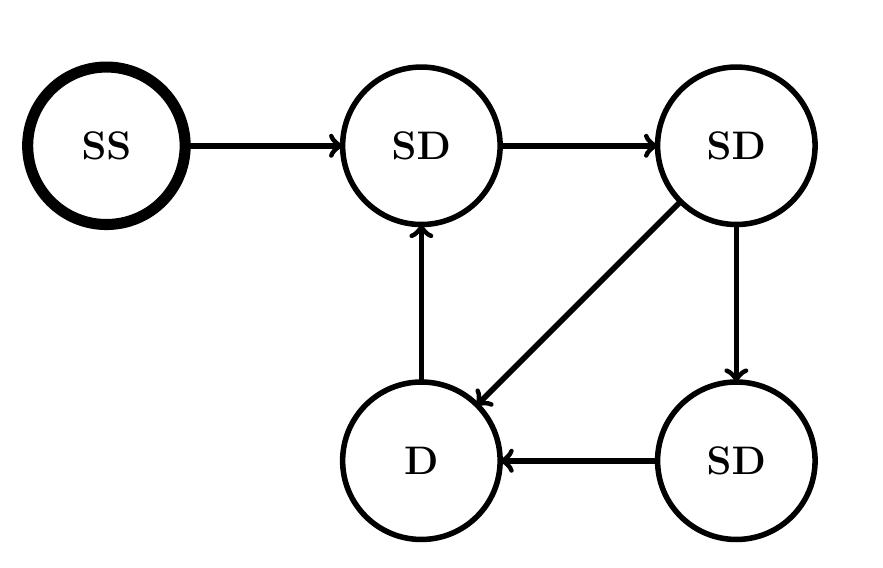
\begin{tikzpicture}   % Begin A100892 series
    
%		\draw[help lines] (0, 0) grid (10,6);
        \useasboundingbox (0, 0) -- (0, 6.5) -- (10.5, 6.5) -- (10.5, 0) -- cycle; 
        
        % Starting Single/Single node for A100892 sequence
        \draw[line width=4] (1,5) circle [radius=1cm];
        \node (start) at (1,5) {\Large \textbf {SS} };
        
        % Single/Double node for A100892 sequence
        \draw[line width=2] (5,5) circle [radius=1cm];
        \node (start) at (5,5) {\Large \textbf {SD} };
        
        % Single/Double node for A100892 sequencee
        \draw[line width=2] (9,5) circle [radius=1cm];
        \node (start) at (9,5) {\Large \textbf {SD} };
        
        % Conditional Single/Double node for A100892 sequence
        \draw[line width=2] (9,1) circle [radius=1cm];
        \node (start) at (9,1) {\Large \textbf {SD} };
        
        % Standalone Double node for A100892 sequence
        \draw[line width=2] (5,1) circle [radius=1cm];
        \node (start) at (5,1) {\Large \textbf {D} };
        
        % Unidirectional arrows between elements in series
        \draw[line width=2,arrows=->] (2,5) -- (4,5);           % SS -> SD
        \draw[line width=2,arrows=->] (6,5) -- (8,5);           % SD -> SD
        \draw[line width=2,arrows=->] (9,4) -- (9,2);           % SD -> SD
        \draw[line width=2,arrows=->] (8,1) -- (6,1);           % SD -> D
        \draw[line width=2,arrows=->] (5,2) -- (5,4);           % D -> SD
        \draw[line width=2,arrows=->] (8.3,4.3) -- (5.7,1.7);   % SD -> S
    
    \end{tikzpicture}   % End A100892 series
	\caption{State Transition Diagram for A186009}
    \label{A100982flow}
\end{figure}



\pagebreak
\subsection{Dropping Time Pattern Sub-cycles}
\label{cyclechoice}
Let's take a moment to examine more closely the impact that \OEIS{A022921} has on \OEIS{A100982} and by extension \OEIS{A186009}.  The final term doubling rule affects the number of new convergent subsequences as the length of the orbit increases.  The complete algorithm is depicted in a flowchart in Figure \ref{subsequences} in Appendix \ref{novel_appendix}.

The sequence \OEIS{A022921} is defined as the number of integers $m$ such that:
\begin{equation}
3^n < 2^m < 3^{n+1}; n \in \setNo,m \in \setN
\label{A022921_definition}
\end{equation}

Which means:
\begin{equation}
\label{A022921_le_unity}
\frac{2^m}{3^{n+1}} < 1; n \in \setNo,m \in \setN
\end{equation}

The \OEIS{A022921} sequence consists of a series of 1's and 2's which are the additional powers of 2 which adhere to the definition as per Equation \ref{A022921_definition}.  Each single (S) or double (D) increments the term from \OEIS{A022921} and therefore represents a single factor of 3.  S indicates a single factor of 2, and D indicates 2 factors of 2.

\pagebreak
% A022921 construction as per the modified recursive algorithm
\begin{center}
    \begin{longtable}{@{}rccccccc|ccccc@{}}
        \label{A022921} \\
        \caption{\OEIS{A022921}$(n)$ Behaviour (7-cycle, 5-cycle)} \\

        \toprule
        $n+$ & 00 & 01 & 02 & 03 & 04 & 05 & 06 & 07 & 08 & 09 & 10 & 11 \\
        
        % Horizontal sum table
        \midrule
           0 & 1 & 2 & 1 & 2 & 1 & 2 & 2 & 1 & 2 & 1 & 2 & 2 \\
          12 & 1 & 2 & 1 & 2 & 1 & 2 & 2 & 1 & 2 & 1 & 2 & 2 \\
          24 & 1 & 2 & 1 & 2 & 1 & 2 & 2 & 1 & 2 & 1 & 2 & 2 \\
          36 & 1 & 2 & 1 & 2 & 1 & 2 & 2 & 1 & 2 & 1 & 2 & 2 \\
          48 & 1 & 2 & 1 & 2 & \color{red}{2} \\
   
        \midrule
          53 & 1 & 2 & 1 & 2 & 1 & 2 & 2 & 1 & 2 & 1 & 2 & 2 \\
          65 & 1 & 2 & 1 & 2 & 1 & 2 & 2 & 1 & 2 & 1 & 2 & 2 \\
          77 & 1 & 2 & 1 & 2 & 1 & 2 & 2 & 1 & 2 & 1 & 2 & 2 \\
          89 & 1 & 2 & 1 & 2 & 1 & 2 & 2 & 1 & 2 & 1 & 2 & 2 \\
         101 & 1 & 2 & 1 & 2 & \color{red}{2}  \\      

        \midrule
          106 & 1 & 2 & 1 & 2 & 1 & 2 & 2 & 1 & 2 & 1 & 2 & 2 \\
          118 & 1 & 2 & 1 & 2 & 1 & 2 & 2 & 1 & 2 & 1 & 2 & 2 \\
        \bottomrule
    \end{longtable}
\end{center}

The 7-cycle SD\Rarr SD\Rarr SD\Rarr D is of length 7 and encompasses 7 powers of 3. This cycle spans 11 powers of 2 with 3 singles and 4 doubles ($3*1+4*2=11$). A 7-cycle overall ratio is thus less than unity at $\frac{2^{11}}{3^{7}} = \frac{2048}{2187} \simeq 0.9364$.

The 5-cycle SD\Rarr SD\Rarr D is of length 5 and encompasses 5 powers of 3.  This cycle spans 8 powers of 2 with 2 singles and 3 doubles ($2*1+3*2=8$). A 5-cycle overall ratio is thus greater than unity at $\frac{2^{8}}{3^{5}} = \frac{256}{243} \simeq 1.0535$.

As per Equation \ref{A022921_le_unity}, the overall ratio of power of 2 divided by power of 3 ($n+1$) for the \OEIS{A022921} sequence must never exceed unity.  The 7-cycle is less than unity and the 5-cycle exceeds unity.  So initially, the patterns begins with a 7-cycle is followed by a 5-cycle, effectively creating the 12-cycle SD\Rarr SD\Rarr SD\Rarr D\Rarr SD\Rarr SD\Rarr D.

The 12-cycle is closer to unity than  the 7-cycle, and contains 12 powers of 3 and 19 powers of 2.  A 12-cycle ratio is thus $\frac{2^{19}}{3^{12}} = \frac{524288}{531441} \simeq 0.9865$.

Since 12-cycles are less than unity, the multiplicative impact of consecutive 12-cycles is to move farther from unity.  After 4 consecutive 12-cycles, the pattern breaks.

% A022921 construction as per the modified recursive algorithm
\begin{center}
    \begin{longtable}{@{}rcccccccccc@{}}
        \label{359_306} \\
        \caption{\OEIS{A022921}$(n)$ Behaviour (53-cycle, 41-cycle)} \\

        \toprule
        $n+$ & 00 & 07 & 12 & 19 & 24 & 31 & 36 & 43 & 48 \\
        
        % Horizontal sum table
        \midrule
            0 & 7 & 5 & 7 & 5 & 7 & 5 & 7 & 5 & 5 \\
           53 & 7 & 5 & 7 & 5 & 7 & 5 & 7 & 5 & 5 \\
          106 & 7 & 5 & 7 & 5 & 7 & 5 & 7 & 5 & 5 \\
          159 & 7 & 5 & 7 & 5 & 7 & 5 & 7 & 5 & 5 \\
          212 & 7 & 5 & 7 & 5 & 7 & 5 & 7 & 5 & 5 \\
          265 & 7 & 5 & 7 & 5 & 7 & 5 & 7 & 5 & 5 \\
          318 & 7 & 5 & 7 & 5 & 7 & 5 & \color{red}{5} \\

        \midrule
          359 & 7 & 5 & 7 & 5 & 7 & 5 & 7 & 5 & 5 \\
          412 & 7 & 5 & 7 & 5 & 7 & 5 & 7 & 5 & 5 \\
          465 & 7 & 5 & 7 & 5 & 7 & 5 & 7 & 5 & 5 \\
          518 & 7 & 5 & 7 & 5 & 7 & 5 & 7 & 5 & 5 \\
          571 & 7 & 5 & 7 & 5 & 7 & 5 & 7 & 5 & 5 \\
          624 & 7 & 5 & 7 & 5 & 7 & 5 & \color{red}{5} \\
   
        \midrule
          665 & 7 & 5 & 7 & 5 & 7 & 5 & 7 & 5 & 5 \\
          718 & 7 & 5 & 7 & 5 & 7 & 5 & 7 & 5 & 5 \\
        \bottomrule
    \end{longtable}
\end{center}

A 48-cycle (7\Rarr 5\Rarr 7\Rarr 5\Rarr 7\Rarr 5\Rarr 7\Rarr5) is $\frac{2^{76}}{3^{48}} = \frac{7.556e22}{7.977e22} \simeq 0.9472$.

Adding a 7-cycle gives $\frac{2^{87}}{3^{55}} = \frac{1.5474e26}{1.7445e26} \simeq 0.8870$ (7\Rarr 5\Rarr 7\Rarr 5\Rarr 7\Rarr 5\Rarr 7\Rarr 5\Rarr 7).

Adding a 5-cycle gives $\frac{2^{84}}{3^{53}} = \frac{1.9343e25}{1.9383e25} \simeq 0.9979$ (7\Rarr 5\Rarr 7\Rarr 5\Rarr 7\Rarr 5\Rarr 7\Rarr 5\Rarr 5).

Therefore, the 53-cycle 7\Rarr 5\Rarr 7\Rarr 5\Rarr 7\Rarr 5\Rarr 7\Rarr 5\Rarr 5 with consecutive 5-cycles at the end is the proper extension to a 48-cycle which is closest to, but less than unity as shown in red in Table \ref{A022921}.   Vertical bars in rows with 12 entries (12-cycles) show 7-cycles followed by 5-cycles.  The term index $n$ of \OEIS{A022921} is the sum of values under $n+$ and the column headings (00 to 11).  The first red 2 is at term $n=48+04=52$.

Since 53-cycle patterns differ from unity by about 0.2\%, this 53-cycle pattern repeats 6 times until three consecutive 12-cycles can be followed by a 5-cycle without exceeding unity.  This extends the pattern with a 41-cycle (3*12+5) which in aggregate can be viewed as a 359-cycle (53*6+41=359) which is closer to unity.

Each 359-cycle is followed by a 306-cycle, effectively making for a 665-cycle.  The 665-cycles pattern repeats until it is possible to fit a 306-cycle without exceeding unity creating a 16266-cycle.  This process of continual pattern refinement is without end as you get ever closer to unity.  Table \ref{359_306} shows where the 7-cycles and 5-cycles are placed in 306, 359 and 665 cycles.

As a consequence of the non-linearity of \OEIS{A186009} and \OEIS{A022921}, performing rigorous algebraic analysis on them directly is not simple.  Instead, we turn to another sequence which has very similar properties to \OEIS{A186009}, but which is much more amenable to algebraic analysis.



\subsection{An introduction to A047749}

There is a very closely related sequence \OEIS{A047749}, which flows as shown in Figure \ref{A04774flow}.  The sequence shares the first few elements of \OEIS{A186009}, but falls behind on the $9^{th}$ term where \OEIS{A047749} has 55 as opposed to \OEIS{A186009} which has 85.  This comes as a result of their being \emph{consecutive} doubles (a double, double) in \OEIS{A186009} whereas in \OEIS{A047749} a double is \emph{always} followed by a single.  From that point onward \OEIS{A047749} has a horizontal sum which is strictly \emph{smaller} and grows \emph{slower} than \OEIS{A186009}.

% This tikz picture object draws the state diagram flow for the algebraic series A047749
\begin{figure}[ht]				% the [ht] places here or top of page
    \centering
    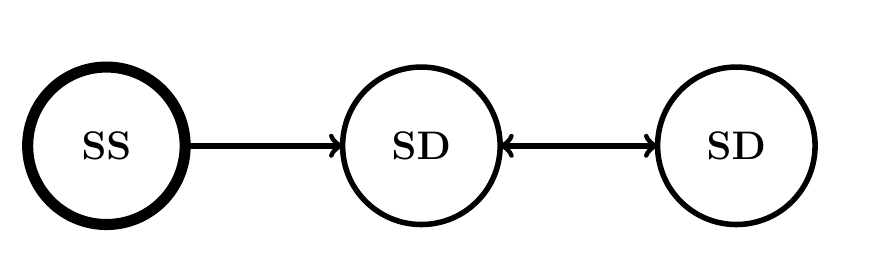
\begin{tikzpicture}
    
%       	\draw[help lines] (0, 0) grid (10,2);
        \useasboundingbox (0, 0) -- (0, 2.5) -- (10.5, 2.5) -- (10.5, 0) -- cycle; 
        
        % Starting Single/Single node for A047749 sequence
        \draw[line width=4] (1,1) circle [radius=1cm];
        \node (start) at (1,1) {\Large \textbf {SS} };
        
        % Single/Double node for A047749 sequence
        \draw[line width=2] (5,1) circle [radius=1cm];
        \node (start) at (5,1) {\Large \textbf {SD} };
        
        % Conditional Single/Double node for A047749 sequence
        \draw[line width=2] (9,1) circle [radius=1cm];
        \node (start) at (9,1) {\Large \textbf {SD} };
        
        % Unidirectional arrow from SS to SD elements in series
        \draw[line width=2,arrows=->] (2,1) -- (4,1);			% SS -> SD

        % Bidirectional arrow from SD back forth to SD elements in series
        \draw[line width=2,arrows=<->] (6,1) -- (8,1);			% SD <-> SD
    
    \end{tikzpicture}   % End A047749 series
	\caption{State Transition Diagram for A047749}
	\label{A04774flow}
\end{figure}

The series \OEIS{A047749} can be generated in much the same way as \OEIS{A186009} with the key exception that the doubling rule is no longer tied to $A022921(n-3) =  2$, which periodically produces consecutive values of 2.  The series \OEIS{A047749} final term doubling goes as per \OEIS{A000034} when $A000034(n) = 2$ for $n \ge 3$.

As a consequence of this, there are never \emph{consecutive} doubles in \OEIS{A047749}, whereas this occurs in \OEIS{A186009}.   Therefore,
\begin{equation}
\label{A186009_ge_A047749_all_n}
A047749(n) \le A186009(n+1); \forall n, n \in \setNo
\end{equation}
 
as shown in Table \ref{A047749} compared with the values in Table \ref{A186009}.  Moreover,
\begin{equation}
\label{A186009_gt_A047749_n_ge_8}
A047749(n) < A186009(n+1); n \ge 8, n \in \setNo
\end{equation}

% A047749 construction as per the modified recursive A100982 algorithm
\begin{center}
	\afterpage{
    \begin{longtable}{@{}rrrrrrrrrrr@{}}
        \label{A047749} \\
        \caption{\OEIS{A047749} Horizontal Sum Formulation} \\

        \toprule
        $n$ & $a_1(n)$ & $a_2(n)$ & $a_3(n)$ & $a_4(n)$ & $a_5(n)$ & $a_6(n)$ & $a_7(n)$ & $a_8(n)$ & $a_9(n)$ & $\sum a_i(n)$ \\
        
        % Horizontal sum table
        \midrule
         0 & 1 &    &     &     &      &      &       &        &       &      1 \\
         1 & 1 &    &     &     &      &      &       &        &       &      1 \\
         2 & 1 &    &     &     &      &      &       &        &       &      1 \\
         3 & 1 &  1 &     &     &      &      &       &        &       &      2 \\
         4 & 1 &  2 &     &     &      &      &       &        &       &      3 \\
         5 & 1 &  3 &   3 &     &      &      &       &        &       &      7 \\
         6 & 1 &  4 &   7 &     &      &      &       &        &       &     12 \\
         7 & 1 &  5 &  12 &  12 &      &      &       &        &       &     30 \\
         8 & 1 &  6 &  18 &  30 &      &      &       &        &       &     55 \\
         9 & 1 &  7 &  25 &  55 &   55 &      &       &        &       &    143 \\
        10 & 1 &  8 &  33 &  88 &  143 &      &       &        &       &    273 \\
        11 & 1 &  9 &  42 & 130 &  273 &  273 &       &        &       &    728 \\
        12 & 1 & 10 &  52 & 182 &  455 &  728 &       &        &       &   1428 \\ 
        13 & 1 & 11 &  63 & 245 &  700 & 1428 &  1428 &        &       &   3876 \\
        14 & 1 & 12 &  75 & 320 & 1020 & 2448 &  3876 &        &       &   7752 \\
        15 & 1 & 13 &  88 & 408 & 1428 & 3876 &  7752 &   7752 &       &  21318 \\
        16 & 1 & 14 & 102 & 510 & 1938 & 5814 & 13566 &  21318 &       &  43263 \\
        17 & 1 & 15 & 117 & 627 & 2565 & 8379 & 21945 &  43263 & 43263 & 120175 \\
        
        \bottomrule
    \end{longtable}
    } % afterpage
\end{center}

Note that the indexing for \OEIS{A186009} begins at $n=1$ whereas the indexing for \OEIS{A047749} begins at $n=0$.  So when the indices for both series are equal then \OEIS{A047749} actually has one \emph{additional} term.

The two sequences are identical for the first 8 terms.  Afterwards, \OEIS{A186009} begins to grow faster, and despite having one extra term $A047749(16) < A100982(16)$.   The gap between the two series accelerates with increasing $n$ due to the periodic \emph{consecutive} doubling effect of \OEIS{A186009}.



\pagebreak
\subsection{Logarithmic derivatives of A047749}
\label{A047749_Convexity}

Since the series \OEIS{A047749} is without the non-linear pattern irregularities inherent in \OEIS{A186009}, it can be probed analytically allowing for determinations to be made as to how this lesser sequence behaves.

The even and odd integer terms of the \OEIS{A047749} sequence can each be separately described in closed form using the discrete binomial formulae provided below.

\begin{define}
Even numbered terms of \OEIS{A047749} sequence are defined as follows:
\begin{equation}
a(n) = \frac{1}{2m+1} \binom{3m}{m}; n = 2m, m \in \setNo
\end{equation}
\end{define}

\begin{define}
Odd numbered terms of \OEIS{A047749} sequence are defined as follows:
\begin{equation}
a(n) = \frac{1}{2m+1} \binom{3m+1}{m+1}; n = 2m+1, m \in \setNo
\end{equation}
\end{define}

Expanding discrete binomial expressions for even and odd members of \OEIS{A047749} into smooth representations using Gamma functions shown in Figure \ref{A047749_Gamma} as per \cite{andrews1985special}:

\begin{figure}[hb]				% the [ht] places here or top of page
	\centering
    % LaTeX cannot follow symbolic links.  Need true directories and files.
    % scales both width and height by 0.38
    \includegraphics[scale=0.38]{./figures/A047749.pdf}
    \caption{Continuous function representation of even/odd terms in \OEIS{A047749}}
    \label{A047749_Gamma}
\end{figure}

For even positive numbers, where $\Gamma{(x})$ is the Gamma function:
\begin{equation}
\label{even_gamma}
a(n) = \frac{1}{2m+1} \binom{3m}{m} = \frac{\Gamma(3m+1)}{\Gamma(2m+2)\Gamma(m+1)}; n = 2m, m \in \setNo
\end{equation}

For odd positive numbers, where $\Gamma{(x})$ is the Gamma function:
\begin{equation}
\label{odd_gamma}
a(n) = \frac{1}{2m+1} \binom{3m+1}{m+1} = \frac{\Gamma(3m+2)}{\Gamma(2m+2)\Gamma(m+2)}; n = 2m+1, m \in \setNo
\end{equation}

\begin{figure}[ht]				% the [ht] places here or top of page
	\centering
    % LaTeX cannot follow symbolic links.  Need true directories and files.
    % scales both width and height by 0.38
    \includegraphics[scale=0.38]{./figures/d_dm_ln_A047749.pdf}
    \caption{First logarithmic derivatives of even/odd functions for \OEIS{A047749}}
\end{figure}

\begin{figure}[ht]				% the [ht] places here or top of page
	\centering
    % LaTeX cannot follow symbolic links.  Need true directories and files.
    % scales both width and height by 0.38
    \includegraphics[scale=0.38]{./figures/d_dm2_ln_A047749.pdf}
    \caption{Second logarithmic derivatives of even/odd functions for \OEIS{A047749}}
\end{figure}

The first logarithmic derivative of the Gamma function is given by:

\begin{equation}
\psi(x) \equiv \frac{d}{dx} ln \left( \Gamma(x) \right)
\end{equation}

And the $n^{th}$ logarithmic derivative of the Gamma function is given by:

\begin{equation}
\psi^{n-1}(x) \equiv \frac{d^n}{dx^n} ln \left( \Gamma(x) \right)
\end{equation}

For even positive numbers ($n=2m$), the first derivative of the logarithm is:
\begin{equation}
\frac{d}{dm} ln \left( \frac{\Gamma(3m+1)}{\Gamma(2m+2)\Gamma(m+1)} \right) = 3 \psi^{0}(3m+1) - 2\psi^{0}(2m+2) - \psi^{0}(m+1)
\end{equation}

For odd positive numbers ($n=2m+1$), the first derivative of the logarithm is:
\begin{equation}
\frac{d}{dm} ln \left( \frac{\Gamma(3m+2)}{\Gamma(2m+2)\Gamma(m+2)} \right) = 3 \psi^{0}(3m+2) - 2\psi^{0}(2m+2) - \psi^{0}(m+2)
\end{equation}

%As an interesting side note, the initial conditions which are injected into the \OEIS{A047749} binomial expressions are similar to the Collatz formulation.  When you evaluate the infinite limit of both the even and odd functions, the first derivatives of the logarithm approach the same value:
%
%\begin{equation}
%\lim_{m \to \infty} \lbrace 3 \psi^{0}(3m+1) - 2\psi^{0}(2m+2) - \psi^{0}(m+1) \rbrace = ln \left(\frac{3^3}{2^2 \cdot 1^1} \right) \simeq 1.9095
%\end{equation}
%
%\begin{equation}
%\lim_{m \to \infty} \lbrace 3 \psi^{0}(3m+2) - 2\psi^{0}(2m+2) - \psi^{0}(m+2) \rbrace = ln \left(\frac{3^3}{2^2 \cdot 1^1} \right) \simeq 1.9095
%\end{equation}

Proceeding now to show that both even and odd \OEIS{A047749} continuous functions are logarithmically convex.  This is accomplished by computing the second derivative of the natural logarithm of the functional representation of the series.

\begin{lemma}
\label{even_lemma}
Even numbers in the sequence \OEIS{A047749} are logarithmically convex.
\end{lemma}

\begin{proof}
For even integers ($n=2m$), the second derivative of the logarithm is:
\begin{equation}
\label{even_convex}
\frac{d^2}{dm^2} ln \left( \frac{\Gamma(3m+1)}{\Gamma(2m+2)\Gamma(m+1)} \right) = 3^2 \psi^{1}(3m+1) - 2^2\psi^{1}(2m+2) - \psi^{1}(m+1)
\end{equation}

Additionally, the limit of the second logarithmic derivative goes to 0 from above.

\begin{equation}
\lim_{m \to \infty} \lbrace 3^2 \psi^{1}(3m+1) - 2^2 \psi^{1}(2m+2) - \psi^{1}(m+1) \rbrace = 0
\end{equation}

The second logarithmic derivative shown in Equation (\ref{even_convex}) has only negative roots and is positive for $m \ge 0$. Thus the logarithm of the function touching all even elements of \OEIS{A047749} is convex.  
\end{proof}

\begin{figure}[ht]				% the [ht] places here or top of page
	\centering
    % LaTeX cannot follow symbolic links.  Need true directories and files.
    % scales both width and height by 0.38
    \includegraphics[scale=0.38]{./figures/A047749_vs_A186009_even.pdf}
    \caption{Comparison of natural log of even function for \OEIS{A047749} versus \OEIS{A186009}}
    \label{even_A047749_vs_A186009}
\end{figure}

\begin{figure}[ht]				% the [ht] places here or top of page
	\centering
    % LaTeX cannot follow symbolic links.  Need true directories and files.
    % scales both width and height by 0.38
    \includegraphics[scale=0.38]{./figures/A047749_vs_A186009_odd.pdf}
    \caption{Comparison of natural log of odd function for \OEIS{A047749} versus \OEIS{A186009}}
    \label{odd_A047749_vs_A186009}
\end{figure}

\pagebreak
\begin{lemma}
\label{odd_lemma}
Odd numbers in the sequence \OEIS{A047749} are logarithmically convex.
\end{lemma}

\begin{proof}
For odd integers ($n=2m+1$), the second derivative of the logarithm is:
\begin{equation}
\label{odd_convex}
\frac{d^2}{dm^2} ln \left( \frac{\Gamma(3m+2)}{\Gamma(2m+2)\Gamma(m+2)} \right) = 3^2 \psi^{1}(3m+2) - 2^2\psi^{1}(2m+2) - \psi^{1}(m+2)
\end{equation}

Additionally, the limit of the second logarithmic derivative goes to 0 from above.

\begin{equation}
\lim_{m \to \infty} \lbrace 3^2 \psi^{1}(3m+2) - 2^2 \psi^{1}(2m+2) - \psi^{1}(m+2) \rbrace = 0
\end{equation}

%\begin{proof}
The second logarithmic derivative shown in Equation (\ref{odd_convex}) has only negative roots and is positive for $m \ge 0$. Thus the logarithm of the function touching all even elements of \OEIS{A047749} is convex.  
\end{proof}

\pagebreak
\begin{theorem}
\label{A047749_convex}
The sequence \OEIS{A047749} is logarithmically convex.
\end{theorem}

\begin{proof}
By Lemma \ref{even_lemma} even numbers in \OEIS{A047749} are logarithmically convex.  By Lemma \ref{odd_lemma} odd numbers in \OEIS{A047749} are logarithmically convex.  Therefore, the entire \OEIS{A047749} sequence is logarithmically convex.
\end{proof}

%\pagebreak
\subsection{Connecting A047749 to A186009}
\label{A186009_Convexity}
%It is important to now leverage the important relation between \OEIS{A047749} and \OEIS{A186009}.

\begin{theorem}
\label{A186009_convex}
The sequence \OEIS{A186009} is logarithmically convex.
\end{theorem}

\begin{proof}
By Theorem \ref{A047749_convex}, the sequence \OEIS{A047749} is logarithmically convex for all positive values.  Since by (\ref{A186009_ge_A047749_all_n}) and (\ref{A186009_gt_A047749_n_ge_8}) the closely related sequence defined by A186009(n+1) is greater than or equal to A047749(n) for $n \in \setNo$ – and strictly greater from the $9^{th}$ term onward, therefore \OEIS{A047749} is also logarithmically convex.
\end{proof}

Theorem \ref{A186009_convex} can be seen by comparing values from Tables \ref{A186009} and \ref{A047749} or via plots comparing \OEIS{A047749} and \OEIS{A186009} for odd and even terms in Figure \ref{even_A047749_vs_A186009} and Figure \ref{odd_A047749_vs_A186009}.

Thus it is established that the \OEIS{A186009} sequence is logarithmically convex.



\newpage
\section{Associative groupings of residuals}
The next very important step is establishing that by using an associative grouping of residuals given by \OEIS{A186009} it is possible to construct collections of residue classes which are $\ge \frac{1}{2^n}$ for all $n$.



\subsection{Associativity of Infinite Series}
There is a well established principle, known as the Associativity of an Infinite Series \cite{Associative_Property}, that states that as long as a series is convergent and you do not change the order of the terms, then an arbitrary grouping of terms produces another series which converges to the same value.

Suppose you have a convergent series of strictly positive terms such that $\sum_{n=1}^{\infty} a_n = L$ and $\sum_{n=1}^k a_n = L_k$ is the partial sum.  Additionally, we define a strictly increasing subsequence of the positive integers $\lbrace n_k \rbrace = \lbrace n_1, n_2, \ldots, n_{k-1}, n_k \rbrace$ serving as term indices (while defining $n_0 = 0$) in the series up to $k$,  for example, $\lbrace 6, 13, 34, 56 \rbrace$.  Now let $b_k = a_{n_{k-1}+1} + a_{n_{k-1}+2} + a_{n_{k-1}+3} + \ldots + a_{n_k}$ such that every term $b_k$ is a regrouping of consecutive terms of the original series without changing the order.

\begin{theorem}
\label{assoc_inf_series}
We assert that $( a_1 + a_2 + \ldots + a_{n_1} ) + ( a_{{n_1}+1} + a_{{n_1}+2} + \ldots + a_{n_2} ) + \ldots + ( a_{n_{k-1}+1} + a_{n_{k-1}+2} + \ldots + a_{n_{k}} ) = L_k$ and $(b_1) + (b_2) + \ldots + (b_k) = L_k$.
\end{theorem}

\begin{proof}
Each sequence of partial sums $S_k = \sum_{i=1}^k b_i$ is identical to the subsequence $s_n = \sum_{i=1}^{n_k} a_i$ and is therefore congruent and so $S_k$\Rarr$L_k$ as $s_n$\Rarr$L_k$. And finally every subsequence of a convergent sequence with a limit $L$ is also convergent and has a limit $L$.  This completes the theorem.
\end{proof}

Using the principle of Associativity of an Infinite Series from Theorem \ref{assoc_inf_series}, it will be shown that a grouping of terms of residual equivalence classes with novel subsequences can be constructed such that these are $\ge \frac{1}{2^n}; \forall n, n \in \setN$.  The $n = 1$ case is straight-forward since this represents the even numbers which each converge to a smaller integer through a single division by 2.



\pagebreak
\subsection{Absolute Cumulative Convergence}
The cumulative convergence, $C(n)$, from Definition \ref{cumulative_convergence} summates all of the individual contributions as novel residues classes are found.  The equation is repeated here for convenience:
\begin{equation}
    C(n) = \sum_{j=0}^n N(j); j,n \in \setNo, C(n) \in \setQ
\end{equation}
The ultimate goal is to prove Proposition \ref{cumulative_convergence_prop} by means of associative grouping of residuals.  The partial sum of Equation \ref{sum_infinite_halves} up to $k$ is:
\begin{equation}
    \sum_{n=1}^k { \frac{1}{ 2^n} } = \frac{2^k-1}{2^k}
\end{equation}
And the previous partial sum up to $k-1$ is:
\begin{equation}
    \sum_{n=1}^{k-1} { \frac{1}{ 2^n} } = \frac{2^{k-1}-1}{2^{k-1}}
\end{equation}
The approach taken is to demonstrate that is it always possible to create groupings of convergent residual classes such that the cumulative portion of the positive integer space is guaranteed to converge to a smaller value over the subsequences is:
\begin{equation}
    C(n) \ge \frac{2^{k-1}-1}{2^{k-1}}
\end{equation}
Recall the formula for the new convergent subsquences from Equation \ref{novel_convergence}:
\begin{equation}
    N(n) = \frac{A186009(n+1)}{2^{A020914(n)}}, n \in \setNo; N(n) \in \setQ
\end{equation} 

\begin{define}
Let $d(n)$ represent the exponent of 2 in the denominator in the convergent subsequence fraction which follows $A020914(n)$.
\begin{equation}
    d(n) = A020914(n);n \in \setNo
\end{equation}
\end{define}
Table \ref{cumulative_0_63} below provides the first 64 novel convergent subsequence lengths which covers subsequences of up to length 100.  It is expanded in full so that it can be later summarized.

% N(n) and C(n)
\begin{center}
    \def\arraystretch{1.5}%  1 is the default, so 1.5 is 50% more
    \begin{longtable}{@{}@{}r@{ }r@{ }c@{ }c@{$>$}c@{}}

        \label{cumulative_0_63} \\
        \caption{Convergence as a function of residual term index} \\

        \toprule
        $n$ & $d(n)$ & $N(n) = \frac{A186009(n+1)}{2^{d(n)}}$ & $C(n) = \sum_0^n N(n)$ & $\frac{2^k-1}{2^k}$ \\
        
        % Novel and cumulative values as a function of n
        \midrule
          0 &   1 & $\frac{A186009(1)}{2^{1}}=\frac{1}{2}$ & $\frac{1}{2}$ & $0$ \\
        \midrule
          1 &   2 & $\frac{A186009(2)}{2^{2}}=\frac{1}{4}$ & $\frac{3}{4}$ & $\frac{1}{2}$ \\
        \midrule
          2 &   4 & $\frac{A186009(3)}{2^{4}}=\frac{1}{16}$ & $\frac{13}{16}$ & $\frac{3}{4}$ \\
          3 &   5 & $\frac{A186009(4)}{2^{5}}=\frac{2}{32}$ & $\frac{28}{32}$ & $\frac{3}{4}$ \\
        \midrule
          4 &   7 & $\frac{A186009(5)}{2^{7}}=\frac{3}{128}$ & $\frac{115}{128}$ & $\frac{7}{8}$ \\
          5 &   8 & $\frac{A186009(6)}{2^{8}}=\frac{7}{256}$ & $\frac{237}{256}$ & $\frac{7}{8}$ \\
          6 &  10 & $\frac{A186009(7)}{2^{10}}=\frac{12}{1024}$ & $\frac{960}{1024}$ & $\frac{7}{8}$ \\
        \midrule
          7 &  12 & $\frac{A186009(8)}{2^{12}}=\frac{30}{4096}$ & $\frac{3870}{4096}$ & $\frac{15}{16}$ \\
          8 &  13 & $\frac{A186009(9)}{2^{13}}=\frac{85}{8192}$ & $\frac{7825}{8192}$ & $\frac{15}{16}$ \\
          9 &  15 & $\frac{A186009(10)}{2^{15}}=\frac{173}{32768}$ & $\frac{31473}{32768}$ & $\frac{15}{16}$ \\
         10 &  16 & $\frac{A186009(11)}{2^{16}}=\frac{476}{65536}$ & $\frac{63422}{65536}$ & $\frac{15}{16}$ \\
        \midrule
         11 &  18 & $\frac{A186009(12)}{2^{18}}=\frac{961}{262144}$ & $\frac{254649}{262144}$ & $\frac{31}{32}$ \\
         12 &  20 & $\frac{A186009(13)}{2^{20}}=\frac{2652}{1048576}$ & $\frac{1021248}{1048576}$ & $\frac{31}{32}$ \\
         13 &  21 & $\frac{A186009(14)}{2^{21}}=\frac{8045}{2097152}$ & $\frac{2050541}{2097152}$ & $\frac{31}{32}$ \\
         14 &  23 & $\frac{A186009(15)}{2^{23}}=\frac{17637}{8388608}$ & $\frac{8219801}{8388608}$ & $\frac{31}{32}$ \\
         15 &  24 & $\frac{A186009(16)}{2^{24}}=\frac{51033}{16777216}$ & $\frac{16490635}{16777216}$ & $\frac{31}{32}$ \\
        \midrule
         16 &  26 & $\frac{A186009(17)}{2^{26}}=\frac{108950}{67108864}$ & $\frac{66071490}{67108864}$ & $\frac{63}{64}$ \\
         17 &  27 & $\frac{A186009(18)}{2^{27}}=\frac{312455}{134217728}$ & $\frac{132455435}{134217728}$ & $\frac{63}{64}$ \\
         18 &  29 & $\frac{A186009(19)}{2^{29}}=\frac{663535}{536870912}$ & $\frac{530485275}{536870912}$ & $\frac{63}{64}$ \\
         19 &  31 & $\frac{A186009(20)}{2^{31}}=\frac{1900470}{2147483648}$ & $\frac{2123841570}{2147483648}$ & $\frac{63}{64}$ \\
         20 &  32 & $\frac{A186009(21)}{2^{32}}=\frac{5936673}{4294967296}$ & $\frac{4253619813}{4294967296}$ & $\frac{63}{64}$ \\
         21 &  34 & $\frac{A186009(22)}{2^{34}}=\frac{13472296}{17179869184}$ & $\frac{17027951548}{17179869184}$ & $\frac{63}{64}$ \\
        \midrule
         22 &  35 & $\frac{A186009(23)}{2^{35}}=\frac{39993895}{34359738368}$ & $\frac{34095896991}{34359738368}$ & $\frac{127}{128}$ \\
         23 &  37 & $\frac{A186009(24)}{2^{37}}=\frac{87986917}{137438953472}$ & $\frac{136471574881}{137438953472}$ & $\frac{127}{128}$ \\
         24 &  39 & $\frac{A186009(25)}{2^{39}}=\frac{257978502}{549755813888}$ & $\frac{546144278026}{549755813888}$ & $\frac{127}{128}$ \\
         25 &  40 & $\frac{A186009(26)}{2^{40}}=\frac{820236724}{1099511627776}$ & $\frac{1093108792776}{1099511627776}$ & $\frac{127}{128}$ \\
         26 &  42 & $\frac{A186009(27)}{2^{42}}=\frac{1899474678}{4398046511104}$ & $\frac{4374334645782}{4398046511104}$ & $\frac{127}{128}$ \\
         27 &  43 & $\frac{A186009(28)}{2^{43}}=\frac{5723030586}{8796093022208}$ & $\frac{8754392322150}{8796093022208}$ & $\frac{127}{128}$ \\
         28 &  45 & $\frac{A186009(29)}{2^{45}}=\frac{12809477536}{35184372088832}$ & $\frac{35030378766136}{35184372088832}$ & $\frac{127}{128}$ \\
        \midrule
         29 &  46 & $\frac{A186009(30)}{2^{46}}=\frac{38036848410}{70368744177664}$ & $\frac{70098794380682}{70368744177664}$ & $\frac{255}{256}$ \\
         30 &  48 & $\frac{A186009(31)}{2^{48}}=\frac{84141805077}{281474976710656}$ & $\frac{280479319327805}{281474976710656}$ & $\frac{255}{256}$ \\
         31 &  50 & $\frac{A186009(32)}{2^{50}}=\frac{248369601964}{1125899906842624}$ & $\frac{1122165646913184}{1125899906842624}$ & $\frac{255}{256}$ \\
         32 &  51 & $\frac{A186009(33)}{2^{51}}=\frac{794919136728}{2251799813685248}$ & $\frac{2245126212963096}{2251799813685248}$ & $\frac{255}{256}$ \\
         33 &  53 & $\frac{A186009(34)}{2^{53}}=\frac{1857112329035}{9007199254740992}$ & $\frac{8982361964181419}{9007199254740992}$ & $\frac{255}{256}$ \\
         34 &  54 & $\frac{A186009(35)}{2^{54}}=\frac{5636545892795}{18014398509481984}$ & $\frac{17970360474255633}{18014398509481984}$ & $\frac{255}{256}$ \\
         35 &  56 & $\frac{A186009(36)}{2^{56}}=\frac{12732900345928}{72057594037927936}$ & $\frac{71894174797368460}{72057594037927936}$ & $\frac{255}{256}$ \\
         36 &  58 & $\frac{A186009(37)}{2^{58}}=\frac{38088111350198}{288230376151711744}$ & $\frac{287614787300824038}{288230376151711744}$ & $\frac{255}{256}$ \\
        \midrule
         37 &  59 & $\frac{A186009(38)}{2^{59}}=\frac{123110229387834}{576460752303423488}$ & $\frac{575352684831035910}{576460752303423488}$ & $\frac{511}{512}$ \\
         38 &  61 & $\frac{A186009(39)}{2^{61}}=\frac{290838337577435}{2305843009213693952}$ & $\frac{2301701577661721075}{2305843009213693952}$ & $\frac{511}{512}$ \\
         39 &  62 & $\frac{A186009(40)}{2^{62}}=\frac{889949312454085}{4611686018427387904}$ & $\frac{4604293104635896235}{4611686018427387904}$ & $\frac{511}{512}$ \\
         40 &  64 & $\frac{A186009(41)}{2^{64}}=\frac{2029460152095008}{18446744073709551616}$ & $\frac{18419201878695679948}{18446744073709551616}$ & $\frac{511}{512}$ \\
         41 &  65 & $\frac{A186009(42)}{2^{65}}=\frac{6113392816333320}{36893488147419103232}$ & $\frac{36844517150207693216}{36893488147419103232}$ & $\frac{511}{512}$ \\
         42 &  67 & $\frac{A186009(43)}{2^{67}}=\frac{13759389839553008}{147573952589676412928}$ & $\frac{147391827990670325872}{147573952589676412928}$ & $\frac{511}{512}$ \\
         43 &  69 & $\frac{A186009(44)}{2^{69}}=\frac{41156292958100112}{590295810358705651712}$ & $\frac{589608468255639403600}{590295810358705651712}$ & $\frac{511}{512}$ \\
         44 &  70 & $\frac{A186009(45)}{2^{70}}=\frac{133180667145777072}{1180591620717411303424}$ & $\frac{1179350117178424584272}{1180591620717411303424}$ & $\frac{511}{512}$ \\
         45 &  72 & $\frac{A186009(46)}{2^{72}}=\frac{315356241137505268}{4722366482869645213696}$ & $\frac{4717715824954835842356}{4722366482869645213696}$ & $\frac{511}{512}$ \\
        \midrule
         46 &  73 & $\frac{A186009(47)}{2^{73}}=\frac{967303800643232882}{9444732965739290427392}$ & $\frac{9436398953710314917594}{9444732965739290427392}$ & $\frac{1023}{1024}$ \\
         47 &  75 & $\frac{A186009(48)}{2^{75}}=\frac{2213388970068123188}{37778931862957161709568}$ & $\frac{37747809203811327793564}{37778931862957161709568}$ & $\frac{1023}{1024}$ \\
         48 &  77 & $\frac{A186009(49)}{2^{77}}=\frac{6687324379116300569}{151115727451828646838272}$ & $\frac{150997924139624427474825}{151115727451828646838272}$ & $\frac{1023}{1024}$ \\
         49 &  78 & $\frac{A186009(50)}{2^{78}}=\frac{21797112395398269352}{302231454903657293676544}$ & $\frac{302017645391644253219002}{302231454903657293676544}$ & $\frac{1023}{1024}$ \\
         50 &  80 & $\frac{A186009(51)}{2^{80}}=\frac{52028134169251235063}{1208925819614629174706176}$ & $\frac{1208122609700746264111071}{1208925819614629174706176}$ & $\frac{1023}{1024}$ \\
         51 &  81 & $\frac{A186009(52)}{2^{81}}=\frac{160509643506854706934}{2417851639229258349412352}$ & $\frac{2416405729044999382929076}{2417851639229258349412352}$ & $\frac{1023}{1024}$ \\
         52 &  83 & $\frac{A186009(53)}{2^{83}}=\frac{369707873749224505928}{9671406556917033397649408}$ & $\frac{9665992624053746756222232}{9671406556917033397649408}$ & $\frac{1023}{1024}$ \\
         53 &  85 & $\frac{A186009(54)}{2^{85}}=\frac{1122428422670255691408}{38685626227668133590597632}$ & $\frac{38665092924637657280580336}{38685626227668133590597632}$ & $\frac{1023}{1024}$ \\
        \midrule
         54 &  86 & $\frac{A186009(55)}{2^{86}}=\frac{3672921591387837707209}{77371252455336267181195264}$ & $\frac{77333858770866702398867881}{77371252455336267181195264}$ & $\frac{2047}{2048}$ \\
         55 &  88 & $\frac{A186009(56)}{2^{88}}=\frac{8808298119720364971552}{309485009821345068724781056}$ & $\frac{309344243381586529960443076}{309485009821345068724781056}$ & $\frac{2047}{2048}$ \\
         56 &  89 & $\frac{A186009(57)}{2^{89}}=\frac{27272844922266198818078}{618970019642690137449562112}$ & $\frac{618715759608095326119704230}{618970019642690137449562112}$ & $\frac{2047}{2048}$ \\
         57 &  91 & $\frac{A186009(58)}{2^{91}}=\frac{63092460692093312467525}{2475880078570760549798248448}$ & $\frac{2474926130893073397791284445}{2475880078570760549798248448}$ & $\frac{2047}{2048}$ \\
         58 &  92 & $\frac{A186009(59)}{2^{92}}=\frac{192189781828748623023765}{4951760157141521099596496896}$ & $\frac{4950044451567975544205592655}{4951760157141521099596496896}$ & $\frac{2047}{2048}$ \\
         59 &  94 & $\frac{A186009(60)}{2^{94}}=\frac{438474769118020519475109}{19807040628566084398385987584}$ & $\frac{19800616281041020197341845729}{19807040628566084398385987584}$ & $\frac{2047}{2048}$ \\
         60 &  96 & $\frac{A186009(61)}{2^{96}}=\frac{1325438036712274130536314}{79228162514264337593543950336}$ & $\frac{79203790562200793063497919230}{79228162514264337593543950336}$ & $\frac{2047}{2048}$ \\
         61 &  97 & $\frac{A186009(62)}{2^{97}}=\frac{4327322846731848749589802}{158456325028528675187087900672}$ & $\frac{158411908447248317975745428262}{158456325028528675187087900672}$ & $\frac{2047}{2048}$ \\
         62 &  99 & $\frac{A186009(63)}{2^{99}}=\frac{10359365401268828714082041}{633825300114114700748351602688}$ & $\frac{633657993154394540731695795089}{633825300114114700748351602688}$ & $\frac{2047}{2048}$ \\
        \midrule
         63 & 100 & $\frac{A186009(64)}{2^{100}}=\frac{32053249939776775765443011}{1267650600228229401496703205376}$ & $\frac{1267348039558728858239157033189}{1267650600228229401496703205376}$ & $\frac{4095}{4096}$ \\
        \bottomrule
    \end{longtable}
\end{center}



\pagebreak
\subsection{Cumulative Convergence Bracketing}
Using the principle of Associativity of an Infinite Series as per Theorem \ref{assoc_inf_series}, we group $C(n)$ results into blocks such that $\frac{2^{k-1}-1}{2^{k-1}} < C(n) \le \frac{2^k-1}{2^k}$.  As can be seen in Table \ref{pascal}, the number of terms required for grouping initially grows in parallel with $\binom{k}{k-2}$.  But then $C(n)$ is seen to grow faster than $\binom{k}{k-2}$ as shown in red beginning when $k=11$.  It requires a smaller value of $n$ to reach the next range than the pure binomial $B = \binom{k}{k-2}$ – it only took 53 terms versus 55 for $k=11$.

The binomial diagonal $0, 1, 3, 6, 10, 15, 21, 28, 36, 45, 55, \ldots$ corresponds to $\binom{k}{k-2}$ beginning with $k=1$. These values match the maximum allowable collection of groupings of convergent subsequences for $C(n) = \sum_0^n N(n) \le \frac{2^k-1}{2^k}$ up to $k=11$ where the diagonal has the value 55 - whereas it only required convergent sub-orbits of up length 53.  Starting with $n=54$ the cumulative sum, $C(n)$, is beyond $\frac{2047}{2048}$.

What is more important is that the differences between the binomial $k-2$ diagonal and the actual requirement grows.  The first differences between the binomial and actual from $k=11$ are $2, 4, 6, 10, 14, 19, 24, 29, 38, 46, 56, 66, 77, 89, \ldots$.  The second differences (suppressing duplicates) illustrates the widening of the gap between binomial and actual which are $0, 2, 4, 5, 7, 8, 10, 11, 12, \ldots$.

The first differences of the \emph{actual} number of terms required to reach the next $\frac{2^k-1}{2^k}$ begins to level off starting at 45. The actual number of terms required to cumulatively extend beyond the next $2^{-k}$ goes as $8, 9, 10, 9, 10, 10, 11, 10, 11, 11, 10, 11, 11, 11, \ldots$ whereas the binomial sequence $\binom{k}{k-2}$ increases linearly.  Therefore the gap between the actual and binomial expression widens as seen in Table \ref{pascal}.

This leads us to the following proposition:

\begin{proposition}
    \label{cumulative_gt_binom_prop}
    \begin{equation}
    	C\binom{k}{k-2} > \frac{2^{k-1}-1}{2^{k-1}}; \forall k, k \in \setNo
    \end{equation} 
\end{proposition}

If this proposition can be validated, then it leads to a definitive argument.

% Table showing that the binomial grouping eventually exceeds the requirements
\begin{center}
	\afterpage{
    \def\arraystretch{1.3}%  1 is the default, so 1.3 is 30% more
    \begin{longtable}{@{}cccc@{$<$}c@{$\le$}ccc@{}}
        \label{pascal} \\
        \caption{Max $C(n)$ convergence value within $\frac{2^{k}-1}{2^{k}}$ range} \\
        \toprule
        $k$ & $\binom{k}{k-2}$ & $n$ & $\frac{2^{k-1}-1}{2^{k-1}}$ & $C(n)$ & $\frac{2^{k}-1}{2^{k}}$ & \\

        
        % Horizontal sum table
        \midrule
         1 &  0 &  0 & 0                   & $C( 0)$ & $\frac{   1}{   2}$ \\
         2 &  1 &  1 & $\frac{   1}{   2}$ & $C( 1)$ & $\frac{   3}{   4}$ \\
         3 &  3 &  3 & $\frac{   3}{   4}$ & $C( 3)$ & $\frac{   7}{   8}$ \\
         4 &  6 &  6 & $\frac{   7}{   8}$ & $C( 6)$ & $\frac{  15}{  16}$ \\
         5 & 10 & 10 & $\frac{  15}{  16}$ & $C(10)$ & $\frac{  31}{  32}$ \\
         6 & 15 & 15 & $\frac{  31}{  32}$ & $C(15)$ & $\frac{  63}{  64}$ \\
         7 & 21 & 21 & $\frac{  63}{  64}$ & $C(21)$ & $\frac{ 127}{ 128}$ \\
         8 & 28 & 28 & $\frac{ 127}{ 128}$ & $C(28)$ & $\frac{ 255}{ 256}$ \\
         9 & 36 & 36 & $\frac{ 255}{ 256}$ & $C(36)$ & $\frac{ 511}{ 512}$ \\
        10 & 45 & 45 & $\frac{ 511}{ 512}$ & $C(45)$ & $\frac{1023}{1024}$ \\
        
        % At 53 is where the grouping pattern diverges from the k choose k-2 binomial
        11 &  55 & {\color{red} 53} & $\frac{  1023}{ 1024}$ & {\color{red}$C(53)$} & $\frac{  2047}{  2048}$ \\
        12 &  66 & {\color{red} 62} & $\frac{  2047}{ 2048}$ & {\color{red}$C( 62)$} & $\frac{  4095}{  4096}$ \\
        13 &  78 & {\color{red} 72} & $\frac{  4095}{ 4096}$ & {\color{red}$C( 72)$} & $\frac{  8191}{  8192}$ \\
        14 &  91 & {\color{red} 81} & $\frac{ 8191}{ 8192}$ & {\color{red}$C( 81)$} & $\frac{ 16383}{ 16384}$ \\
        15 & 105 & {\color{red} 91} & $\frac{16383}{16384}$ & {\color{red}$C( 91)$} & $\frac{ 32767}{ 32768}$ \\
        16 & 120 & {\color{red}101} & $\frac{32767}{32768}$ & {\color{red}$C(101)$} & $\frac{ 65535}{ 65536}$ \\
        17 & 136 & {\color{red}112} & $\frac{65535}{65536}$ & {\color{red}$C(112)$} & $\frac{131071}{131072}$ \\
        18 & 153 & {\color{red}122} & $\frac{131071}{131072}$ & {\color{red}$C(122)$} & $\frac{262143}{262144}$ \\
        19 & 171 & {\color{red}133} & $\frac{262143}{262144}$ & {\color{red}$C(133)$} & $\frac{524287}{524288}$ \\
        20 & 190 & {\color{red}144} & $\frac{524287}{524288}$ & {\color{red}$C(144)$} & $\frac{1048575}{1048576}$ \\
        21 & 210 & {\color{red}154} & $\frac{1048575}{1048576}$ & {\color{red}$C(154)$} & $\frac{2097151}{2097152}$ \\
        22 & 231 & {\color{red}165} & $\frac{2097151}{2097152}$ & {\color{red}$C(165)$} & $\frac{4194303}{4194304}$ \\
        23 & 253 & {\color{red}176} & $\frac{4194303}{4194304}$ & {\color{red}$C(176)$} & $\frac{8388607}{8388608}$ \\
        24 & 276 & {\color{red}187} & $\frac{8388607}{8388608}$ & {\color{red}$C(187)$} & $\frac{16777215}{16777216}$ \\

        \bottomrule
    \end{longtable}
    } % afterpage
\end{center}


\newpage
\section{Numerical Analysis}

There remain areas of interest which are resistant to algebraic analysis.  Growth rate of some series as well as incremental and cumulative convergence from sequences with finite stopping times follow a non-linear trajectory.  Numerical analysis is often the least preferred avenue, but nevertheless it is called upon to provide conclusive evidence allowing us to draw a number of important conclusions.



\subsection{Consecutive Ratios of Novel Convergence Factors}
We begin with a verbose table computing the ratio of consecutive novel convergence factors $N(n)$, showing how consecutive ratios change over the first five 53-cycles and another distant one.  The calculated values are truncated to 5 decimals (no rounding is performed) so as not to over-estimate the ratios.  It's evident that the consecutive ratios increase from left to right across each of the rows.

% 53-cycle column ratios between current and next term fractions - truncated to 5 decimals
\begin{center}
%    \setlength\tabcolsep{2pt}
    \small
    \begin{longtable}{@{}rcccccc@{}}
        \label{consecutive_ratios_53_5} \\
        \caption{$\frac{N(n)}{N(n-1)}$ ratio (truncated to 5 decimals)} \\

        \toprule        
        $n+$ &   00    &   53    &   106   &   159   &   212   &  79800 \\
        
        % Consecutive ratio table
        \midrule
           0 & 0.50000 & 0.75899 & 0.76926 & 0.77270 & 0.77443 & 0.77961 \\
           1 & 0.50000 & 1.63614 & 1.65517 & 1.66162 & 1.66487 & 1.67470 \\
           2 & 0.25000 & 0.59954 & 0.60827 & 0.61127 & 0.61278 & 0.61739 \\
           3 & 1.00000 & 1.54813 & 1.56635 & 1.57269 & 1.57590 & 1.58574 \\
           4 & 0.37500 & 0.57834 & 0.58681 & 0.58978 & 0.59130 & 0.59597 \\
           5 & 1.16666 & 1.52308 & 1.54087 & 1.54719 & 1.55043 & 1.56046 \\
           6 & 0.42857 & 0.57036 & 0.57862 & 0.58159 & 0.58312 & 0.58788 \\
           7 & 0.62500 & 0.75570 & 0.76439 & 0.76754 & 0.76917 & 0.77428 \\
           8 & 1.41666 & 1.63241 & 1.64851 & 1.65442 & 1.65749 & 1.66717 \\
           9 & 0.50882 & 0.59848 & 0.60588 & 0.60862 & 0.61005 & 0.61459 \\
          10 & 1.37572 & 1.54706 & 1.56253 & 1.56833 & 1.57136 & 1.58104 \\
          11 & 0.50472 & 0.57818 & 0.58538 & 0.58810 & 0.58953 & 0.59412 \\

        \midrule
          12 & 0.68990 & 0.76168 & 0.76926 & 0.77215 & 0.77368 & 0.77860 \\
          13 & 1.51677 & 1.64139 & 1.65548 & 1.66091 & 1.66378 & 1.67313 \\
          14 & 0.54807 & 0.60202 & 0.60852 & 0.61104 & 0.61238 & 0.61676 \\
          15 & 1.44675 & 1.55347 & 1.56708 & 1.57241 & 1.57526 & 1.58462 \\
          16 & 0.53372 & 0.58087 & 0.58721 & 0.58972 & 0.59107 & 0.59551 \\
          17 & 1.43393 & 1.52849 & 1.54187 & 1.54720 & 1.55008 & 1.55962 \\
          18 & 0.53090 & 0.57290 & 0.57914 & 0.58164 & 0.58300 & 0.58752 \\
          19 & 0.71603 & 0.75840 & 0.76498 & 0.76765 & 0.76909 & 0.77395 \\
          20 & 1.56189 & 1.63745 & 1.64968 & 1.65469 & 1.65741 & 1.66662 \\
          21 & 0.56733 & 0.60081 & 0.60644 & 0.60877 & 0.61004 & 0.61435 \\
          22 & 1.48430 & 1.55195 & 1.56378 & 1.56869 & 1.57139 & 1.58059 \\
          23 & 0.55000 & 0.58046 & 0.58598 & 0.58829 & 0.58957 & 0.59393 \\

        \midrule
          24 & 0.73300 & 0.76408 & 0.76991 & 0.77237 & 0.77373 & 0.77842 \\
          25 & 1.58973 & 1.64586 & 1.65673 & 1.66136 & 1.66392 & 1.67281 \\
          26 & 0.57894 & 0.60409 & 0.60911 & 0.61126 & 0.61245 & 0.61663 \\
          27 & 1.50647 & 1.55779 & 1.56835 & 1.57290 & 1.57544 & 1.58435 \\
          28 & 0.55955 & 0.58288 & 0.58782 & 0.58996 & 0.59116 & 0.59539 \\
          29 & 1.48471 & 1.53273 & 1.54317 & 1.54774 & 1.55030 & 1.55938 \\
          30 & 0.55302 & 0.57488 & 0.57976 & 0.58190 & 0.58311 & 0.58742 \\
          31 & 0.73794 & 0.76049 & 0.76564 & 0.76793 & 0.76922 & 0.77385 \\
          32 & 1.60027 & 1.64132 & 1.65094 & 1.65524 & 1.65767 & 1.66644 \\
          33 & 0.58405 & 0.60259 & 0.60703 & 0.60903 & 0.61016 & 0.61427 \\
          34 & 1.51755 & 1.55568 & 1.56503 & 1.56925 & 1.57166 & 1.58043 \\
          35 & 0.56474 & 0.58229 & 0.58657 & 0.58856 & 0.58970 & 0.59386 \\

        \midrule
          36 & 0.74782 & 0.76591 & 0.77054 & 0.77266 & 0.77388 & 0.77835 \\
          37 & 1.61612 & 1.64927 & 1.65792 & 1.66191 & 1.66420 & 1.67268 \\
          38 & 0.59060 & 0.60566 & 0.60966 & 0.61152 & 0.61259 & 0.61657 \\
          39 & 1.52997 & 1.56109 & 1.56953 & 1.57346 & 1.57574 & 1.58423 \\
          40 & 0.57010 & 0.58442 & 0.58838 & 0.59023 & 0.59131 & 0.59534 \\
          41 & 1.50616 & 1.53598 & 1.54436 & 1.54831 & 1.55061 & 1.55928 \\
          42 & 0.56267 & 0.57639 & 0.58032 & 0.58218 & 0.58326 & 0.58737 \\
          43 & 0.74778 & 0.76208 & 0.76624 & 0.76822 & 0.76938 & 0.77380 \\
          44 & 1.61798 & 1.64429 & 1.65207 & 1.65579 & 1.65798 & 1.66635 \\
          45 & 0.59197 & 0.60396 & 0.60756 & 0.60929 & 0.61031 & 0.61423 \\
          46 & 1.53366 & 1.55855 & 1.56614 & 1.56981 & 1.57198 & 1.58035 \\
          47 & 0.57205 & 0.58354 & 0.58710 & 0.58883 & 0.58985 & 0.59382 \\

        \midrule
          48 & 0.75532 & 0.76733 & 0.77110 & 0.77295 & 0.77404 & 0.77831 \\
          49 & 1.62973 & 1.65192 & 1.65898 & 1.66245 & 1.66451 & 1.67261 \\
          50 & 0.59673 & 0.60688 & 0.61015 & 0.61177 & 0.61274 & 0.61654 \\
          51 & 1.54252 & 1.56366 & 1.57057 & 1.57400 & 1.57605 & 1.58417 \\
          52 & 0.57583 & 0.58563 & 0.58887 & 0.59049 & 0.59146 & 0.59531 \\

        \bottomrule
    \end{longtable}
\end{center}
%
%% 53-cycle column ratios between current and next term fractions - truncated to 4 decimals
%\begin{center}
%%    \setlength\tabcolsep{2pt}
%    \small
%    \begin{longtable}{@{}rcccccc@{}}
%        \label{consecutive_ratios_53_4} \\
%        \caption{$\frac{N(n)}{N(n-1)}$ ratio (truncated to 4 decimals)} \\
%
%        \toprule        
%        $n+$ &   00   &   53   &  106   &  159   &  212   & 79853 \\
%        
%        % Consecutive ratio table
%        \midrule
%           0 & 0.5000 & 0.7589 & 0.7692 & 0.7727 & 0.7744 & 0.7796 \\
%           1 & 0.5000 & 1.6361 & 1.6551 & 1.6616 & 1.6648 & 1.6747 \\
%           2 & 0.2500 & 0.5995 & 0.6082 & 0.6112 & 0.6127 & 0.6173 \\
%           3 & 1.0000 & 1.5481 & 1.5663 & 1.5726 & 1.5759 & 1.5857 \\
%           4 & 0.3750 & 0.5783 & 0.5868 & 0.5897 & 0.5913 & 0.5959 \\
%           5 & 1.1666 & 1.5230 & 1.5408 & 1.5471 & 1.5504 & 1.5604 \\
%           6 & 0.4285 & 0.5703 & 0.5786 & 0.5815 & 0.5831 & 0.5878 \\
%           7 & 0.6250 & 0.7557 & 0.7643 & 0.7675 & 0.7691 & 0.7742 \\
%           8 & 1.4166 & 1.6324 & 1.6485 & 1.6544 & 1.6574 & 1.6671 \\
%           9 & 0.5088 & 0.5984 & 0.6058 & 0.6086 & 0.6100 & 0.6145 \\
%          10 & 1.3757 & 1.5470 & 1.5625 & 1.5683 & 1.5713 & 1.5810 \\
%          11 & 0.5047 & 0.5781 & 0.5853 & 0.5881 & 0.5895 & 0.5941 \\
%
%        \midrule
%          12 & 0.6899 & 0.7616 & 0.7692 & 0.7721 & 0.7736 & 0.7786 \\
%          13 & 1.5167 & 1.6413 & 1.6554 & 1.6609 & 1.6637 & 1.6731 \\
%          14 & 0.5480 & 0.6020 & 0.6085 & 0.6110 & 0.6123 & 0.6167 \\
%          15 & 1.4467 & 1.5534 & 1.5670 & 1.5724 & 1.5752 & 1.5846 \\
%          16 & 0.5337 & 0.5808 & 0.5872 & 0.5897 & 0.5910 & 0.5955 \\
%          17 & 1.4339 & 1.5284 & 1.5418 & 1.5472 & 1.5500 & 1.5596 \\
%          18 & 0.5309 & 0.5729 & 0.5791 & 0.5816 & 0.5830 & 0.5875 \\
%          19 & 0.7160 & 0.7584 & 0.7649 & 0.7676 & 0.7690 & 0.7739 \\
%          20 & 1.5618 & 1.6374 & 1.6496 & 1.6546 & 1.6574 & 1.6666 \\
%          21 & 0.5673 & 0.6008 & 0.6064 & 0.6087 & 0.6100 & 0.6143 \\
%          22 & 1.4843 & 1.5519 & 1.5637 & 1.5686 & 1.5713 & 1.5805 \\
%          23 & 0.5500 & 0.5804 & 0.5859 & 0.5882 & 0.5895 & 0.5939 \\
%
%        \midrule
%          24 & 0.7330 & 0.7640 & 0.7699 & 0.7723 & 0.7737 & 0.7784 \\
%          25 & 1.5897 & 1.6458 & 1.6567 & 1.6613 & 1.6639 & 1.6728 \\
%          26 & 0.5789 & 0.6040 & 0.6091 & 0.6112 & 0.6124 & 0.6166 \\
%          27 & 1.5064 & 1.5577 & 1.5668 & 1.5729 & 1.5754 & 1.5843 \\
%          28 & 0.5595 & 0.5828 & 0.5878 & 0.5899 & 0.5911 & 0.5953 \\
%          29 & 1.4847 & 1.5327 & 1.5431 & 1.5477 & 1.5503 & 1.5593 \\
%          30 & 0.5530 & 0.5748 & 0.5797 & 0.5819 & 0.5831 & 0.5874 \\
%          31 & 0.7379 & 0.7604 & 0.7656 & 0.7679 & 0.7692 & 0.7738 \\
%          32 & 1.6002 & 1.6413 & 1.6509 & 1.6552 & 1.6576 & 1.6664 \\
%          33 & 0.5840 & 0.6025 & 0.6070 & 0.6090 & 0.6101 & 0.6142 \\
%          34 & 1.5175 & 1.5556 & 1.5650 & 1.5692 & 1.5716 & 1.5804 \\
%          35 & 0.5647 & 0.5822 & 0.5865 & 0.5885 & 0.5897 & 0.5938 \\
%
%        \midrule
%          36 & 0.7478 & 0.7659 & 0.7705 & 0.7726 & 0.7738 & 0.7783 \\
%          37 & 1.6161 & 1.6492 & 1.6579 & 1.6619 & 1.6642 & 1.6726 \\
%          38 & 0.5906 & 0.6056 & 0.6096 & 0.6115 & 0.6125 & 0.6165 \\
%          39 & 1.5299 & 1.5610 & 1.5669 & 1.5734 & 1.5757 & 1.5842 \\
%          40 & 0.5701 & 0.5844 & 0.5883 & 0.5902 & 0.5913 & 0.5953 \\
%          41 & 1.5061 & 1.5359 & 1.5443 & 1.5483 & 1.5506 & 1.5592 \\
%          42 & 0.5626 & 0.5763 & 0.5803 & 0.5821 & 0.5832 & 0.5873 \\
%          43 & 0.7477 & 0.7620 & 0.7662 & 0.7682 & 0.7693 & 0.7738 \\
%          44 & 1.6179 & 1.6442 & 1.6520 & 1.6557 & 1.6579 & 1.6663 \\
%          45 & 0.5919 & 0.6039 & 0.6075 & 0.6092 & 0.6103 & 0.6142 \\
%          46 & 1.5336 & 1.5585 & 1.5661 & 1.5698 & 1.5719 & 1.5803 \\
%          47 & 0.5720 & 0.5835 & 0.5870 & 0.5888 & 0.5898 & 0.5938 \\
%
%        \midrule
%          48 & 0.7553 & 0.7673 & 0.7711 & 0.7729 & 0.7740 & 0.7783 \\
%          49 & 1.6297 & 1.6519 & 1.6589 & 1.6624 & 1.6645 & 1.6726 \\
%          50 & 0.5967 & 0.6068 & 0.6101 & 0.6117 & 0.6127 & 0.6165 \\
%          51 & 1.5425 & 1.5636 & 1.5705 & 1.5740 & 1.5760 & 1.5841 \\
%          52 & 0.5758 & 0.5856 & 0.5888 & 0.5904 & 0.5914 & 0.5953 \\
%
%        \bottomrule
%    \end{longtable}
%\end{center}

The purpose is to endeavor to establish Proposition \ref{cumulative_gt_binom_prop} by showing that each successive grouping of residual class fractions covers the next $\frac{1}{2^k}$ interval without requiring more than $\binom{k}{k-2}$ terms.  The simplest way to accomplish goal would be if each term in the next grouping is $\ge$ 50\% of the term(s) preceding it.

The series of fractions starts out this way since the sequence begins with the even numbers which represent $\frac{1}{2}$ of the positive integers, allowing $N(-1)=1$ as the boundary condition representing all positive integers. Thus the grouping of terms in Table \ref{pascal} for $k=1$ contains only one element $N(0)$ representing the even numbers.

The next interval is $\frac{1}{4}$ which is also exactly 50\% of the prior term of $\frac{1}{2}$.  This becomes the second column entry in Table \ref{consecutive_ratios_53_5} - representing the ratio of the $n=1$ fraction over the $n=0$ fraction and represents half of the odd positive integers.  Thus the grouping of terms in Table \ref{pascal} for $k=2$ also contains only one element $N(1)$.

However, the ratio of the $n=2$ term over the $n=1$ entry is $\frac{1}{4}$ in Table \ref{consecutive_ratios_53_5} which is less than 50\% so it requires additional term(s) so that the sum of those terms cover the next $\frac{1}{2^k}$ bracket.  The $n=3$ term happens to be equal to the $n=2$ term (consecutive ratio=1.0), and as a result the sum of the two terms is sufficient and seen in Table \ref{pascal} for $n=3$.

And it continues where it is observed that each new grouping requires one additional term beyond the previous $\frac{1}{2^k}$ bracket.  At $k=11$, this linear growth pattern breaks down, requiring fewer cumulative convergence terms than $k-2$ binomial produced, shown in red in Table \ref{pascal}.

%As mentioned earlier, the ratios of the consecutive terms grows in each row in the 53-cycle as shown in Table \ref{consecutive_ratios_53_5}.  Within each row the ratio increases monotonically due to the logarithmic convexity of \OEIS{A186009} as per Theorem \ref{A186009_convex}.



\subsection{Term Growth Impedance}
It is time to examine the forces which provide impedance to the growth in the number of terms required to cover the next $2^{-k}$ bracket.

% Place all floats together with one figure at the top and force another figure below

\begin{figure}[ht]				% the [ht] places here or top of page
    \centering
    % LaTeX cannot follow symbolic links.  Need true directories and files.
    % scales both width and height by 0.48
    \includegraphics[scale=0.48]{./figures/11_term_brackets.pdf}
    \caption{Ratio of $\sum{11-term}$ to $2^k$ bracket}
    \label{11_term_coverage}
\end{figure}

\begin{figure}[!hb]				% forces [!hb] places here or bottom of page
    \centering
    % LaTeX cannot follow symbolic links.  Need true directories and files.
    % scales both width and height by 0.48
    \includegraphics[scale=0.48]{./figures/12_term_brackets.pdf}
    \caption{Ratio of $\sum{12-term}$ to $2^k$ bracket}
    \label{12_term_coverage}
\end{figure}

\begin{figure}[ht]				% the [ht] places here or top of page
    \centering
    % LaTeX cannot follow symbolic links.  Need true directories and files.
    % scales both width and height by 0.48
    \includegraphics[scale=0.48]{./figures/13_term_brackets.pdf}
    \caption{Ratio of $\sum{13-term}$ to $2^k$ bracket}
    \label{13_term_coverage}
\end{figure}

\begin{figure}[!hb]				% forces [!hb] places here or bottom of page
    \centering
    % LaTeX cannot follow symbolic links.  Need true directories and files.
    % scales both width and height by 0.48
    \includegraphics[scale=0.48]{./figures/14_term_brackets.pdf}
    \caption{Ratio of $\sum{14-term}$ to $2^k$ bracket}
    \label{14_term_coverage}
\end{figure}

It is observed that term groupings which cover $2^{-k}$ starting from a single term through 10-term summations cease for $n>154$.  Instead we begin our analysis with the emergence of 11-term coverage.  Figure \ref{11_term_coverage}a) shows the occurrences and \ref{11_term_coverage}b) provides a histogram of the ratio of the 11-term sum to the subsequent $2^{-k}$ bracket.  A ratio in excess of 1 or more indicates that the 11-term sum was greater than $2^{-k}$.

As is evident Figure \ref{11_term_coverage}a), as $n$ increases the ratio of the sum of 11 novel convergence classes, $N(n)$, (Equation \ref{novel_convergence}) declines from above unity to below unity.  Eventually, the ratio decreases to the point that cumulative convergence, C(n), (Equation \ref{cumulative_convergence}) utilizing 11-term summations are insufficient to cover any new $2^{-k}$ brackets.  The last occurrence observed (up to $n=80000$) was found at $n=492$.

Turning attention to the 12-term summations shown in Figure \ref{12_term_coverage}, we see a very different behavior.  While it is clear in Figure \ref{12_term_coverage}a) that there is an obviously declining ratios for larger values of $n$, the rate of change flattens significantly such that 12-term coverage of new $2^{-k}$ brackets still occurs up to $n=80000$.  Note, however, that \ref{12_term_coverage}b) shows a strong indication that 12-term summations ratios to $2^{-k}$ brackets are primarily less than unity meaning that longer summations are required since 12-term summations alone cannot provide limitless recurring $2^{-k}$ bracket coverage.

Examining 13-term summations we see some similar behaviour to the 12-term solutions.  However with 13-terms summations we can clearly see in Figure \ref{13_term_coverage}a) that there are several \emph{families} of solutions and that each of these exhibit the same consecutive ratio flattening observed with the 12-term solutions.

What becomes evident is the emergence of two consecutive ratio modes which the histogram \ref{13_term_coverage}b) illustrates.  It is also clear is that the large majority of the 13-term summation ratios are in excess of unity relative to a new $2^{-k}$ bracket.  Thus 13-term summations in combination with 12-term summations can provide bracket coverage as is observed up to $n=80000$.

Lastly, we look for the existence of 14-term summations - and we find that 14-term solutions do in fact occur as seen in Figure \ref{14_term_coverage}.  It is evident, however, that up to $n=80000$, 14-term summations are uncommon.  All of the 14-term summations found up to $n=80000$ are sandwiched between two 12-term summations.  So in a sense, these 14-term summation solutions are not entirely distinct from 12-term coverage followed by consecutive 13-term summations.  What is also very obvious in \ref{14_term_coverage}b) is the two modes and that all 14-term summations are all in excess of unity.

No 15-term summations occurred up to $n=80000$.

\begin{figure}[ht]				% the [ht] places here or top of page
    \centering
    % LaTeX cannot follow symbolic links.  Need true directories and files.
    % scales both width and height by 0.6
    \includegraphics[scale=0.6]{./figures/Cn_vs_Bk.pdf}
    \caption{Natural logarithms of the maximum cumulative convergence $C(n)$ as compared to the binomial $B(k)=\binom{k}{k-2}$ coefficients}
    \label{cn_bk}
\end{figure}

Figure \ref{cn_bk} shows the rate of growth of both the cumulative convergence function $C(n)$ and the binomial $\binom{k}{k-2}$.  By $n=80000$ (corresponding to $k=6367$), the difference between the logarithmic curves is excess of 5.53, so that the value $B(k) = \binom{k}{k-2}$ is over $e^{5.53} \simeq 250$ \emph{times} the value of $C(n=80000)$.  


\subsection{Detailed investigation into 13-term family}
A quick look at the small piece of the 13-summation shown in Figure \ref{13_term_coverage}.  There is a conspicuous line which is less than unity which appears as if it is from a single source.  However on closer examination we find that some of the data points originate from a 13-term sequence beginning at term 30 and ending at term 42 of a 53-cycle.  The very last data point shown below originates from the data shown in the 79800 column in Table \ref{consecutive_ratios_53_5}.

However embedded within this series is other data which is similar - but differentiated since it begins at term 18 and ends at term 31 of a 41-cycle.  These two data set are plot together on the graph below but in distinct colours and it is obvious that the data sets are distinct.

\begin{figure}[ht]				% the [ht] places here or top of page
    \centering
    % LaTeX cannot follow symbolic links.  Need true directories and files.
    \includegraphics[width=\linewidth]{./figures/best_fit_31_43.pdf}
    \caption{Detail of 13-term summation for ratios $< 0.993$}
    \label{31-43-ratios}
\end{figure}

Also note that a linear curve of best fit was computed and plotted along with the two set of data points.  In either case, there remains some residual negative slope on the order of $10^{-9}$.

A linear fit does not presume that the data is approaching a horizontal asymptote which may or may not exist.  Given that the data point pattern suggests that new lower values are being found a linear fit would appear to be a reasonable choice.


\subsection{Consecutive Term Summation Ratios}

In order to disambiguate whether the rate of term growth required to cover the subsequent $2^{-k}$ brackets merely slows - or stops completely, we compute the ratios of n-terms summations over the prior n-term summation.

If ever we find that this ratio exceeds $\frac{1}{2}$ then we have confirmation that the next n-term summation covers the next $2^{-k}$ bracket - presuming of course that the prior bracket did also.  This ratio was computed up to $n=80000$ for 10, 11, 12, 13, 14 and 15 term summations.  In order to plot the results with improved resolution the first 500 ratios of each type were omitted which eliminated the early transients.

\begin{figure}[ht]				% the [ht] places here or top of page
    \centering
    % LaTeX cannot follow symbolic links.  Need true directories and files.
    \includegraphics[width=\linewidth]{./figures/12_Term_Group_Ratios.pdf}
    \caption{Ratio of 12-term sum divided by prior 12-term sum}
    \label{12-term-group-ratios}
\end{figure}

\begin{figure}[ht]				% the [ht] places here or top of page
    \centering
    % LaTeX cannot follow symbolic links.  Need true directories and files.
    \includegraphics[width=\linewidth]{./figures/13_Term_Group_Ratios.pdf}
    \caption{Ratio of 13-term sum divided by prior 13-term sum}
    \label{13-term-group-ratios}
\end{figure}

The ratios of 10-term and 11-term summations were plotted (Appendix \ref{auxiliary_graphics})and indeed exceeded $\frac{1}{2}$, however beyond the initial values these sums do not cover the next $2^{-k}$ bracket and therefore do not occur after $n=500$.  The 12-term summations by themselves are also insufficient as seen in Figure \ref{12_term_coverage}a) beyond $n=600$.

The majority of 13-term consecutive ratios are however sufficient as shown in \ref{13_term_coverage}a) and indeed that is primary mode where consecutive ratios straddle $\frac{1}{2}$ shown in Figure \ref{13-term-group-ratios}.  We also observe from Figure \ref{13_term_coverage}a) that the majority of 13-term summations exceed the required $2^{-k}$ bracket.

Most 13-term summations cover the bracket with some excess.  This means that the subsequent $2^{-k}$ bracket requires a lesser amount to complete the coverage.  Indeed we find that 12-term summations are required to be part of the sequence since excessive consecutive 13-term summations would exceed what is required to cover the next bracket.

Note that both 14-term and 15-term summations were plotted as well (Appendix \ref{auxiliary_graphics}) and these ratios are all \emph{less} than $\frac{1}{2}$ however both 14 and 15 term summations far exceed what is required for $2^{-k}$ and indeed 14-term summations are observed to be rather uncommon (and have 12-term summations before and after) in the sequence and 15-terms summation are absent entirely up to $n=80000$.

Since 14-term summations are always greater than what is needed to cover the next $2^{-k}$ bracket this becomes the term growth barrier.  It means that 15-term summations can never occur because of the shadowing effect of the 14-term summations.

%\begin{figure}[ht]
%    \centering
%    \begin{tikzpicture}[node distance=0.5cm, every node/.style={draw, align=center, minimum width=3cm, rounded corners}]
%    
%        % Define nodes with A1, A2, B1, B2 format
%        \node (A1) {71810.0, 0.5271153};
%        \node (A2) [right=of A1] {72940.0, 0.5270952};
%        \node (B1) [below=of A1] {73140.0, 0.5271179};
%        \node (B2) [below=of A2] {74270.0, 0.5270976};
%        \node (C1) [below=of B1] {74470.0, 0.5271203};
%        \node (C2) [below=of B2] {75600.0, 0.5271000};
%        \node (D1) [below=of C1] {75800.0, 0.5271227};
%        \node (D2) [below=of C2] {76930.0, 0.5271023};
%        \node (E1) [below=of D1] {77130.0, 0.5271250};
%        \node (E2) [below=of D2] {78260.0, 0.5271046};
%        \node (F1) [below=of E1] {78460.0, 0.5271272};
%        \node (F2) [below=of E2] {79590.0, 0.5271067};
%        \node (G1) [below=of F1] {79790.0, 0.5271294};
%        \node (G2) [below=of F2] {79990.0, 0.5273653};
%    
%        % Draw thicker downward arrows
%        \foreach \X/\Y in {A1/B1, B1/C1, C1/D1, D1/E1, E1/F1, F1/G1} {
%            \draw[->, line width=1mm] (\X) -- (\Y);
%        }
%    
%        \foreach \X/\Y in {A2/B2, B2/C2, C2/D2, D2/E2, E2/F2, F2/G2} {
%            \draw[->, line width=1mm] (\X) -- (\Y);
%        }
%
%    \end{tikzpicture}
%    \caption{Logarithmic convexity effect on 13-term upper bound summations}
%    \label{upper_log_convexity}
%\end{figure}
%
%\begin{figure}[ht]
%    \centering
%    \begin{tikzpicture}[node distance=0.5cm, every node/.style={draw, align=center, minimum width=3cm, rounded corners}]
%    
%        % Define nodes for three columns (equal lengths)
%        \node (A1) {71290.0, 0.4554110};
%        \node (A2) [right=of A1] {71490.0, 0.4554383};
%        \node (A3) [right=of A2] {71690.0, 0.4558649};
%
%        \node (B1) [below=of A1] {72620.0, 0.4554133};
%        \node (B2) [below=of A2] {72820.0, 0.4554405};
%        \node (B3) [below=of A3] {73020.0, 0.4558671};
%
%        \node (C1) [below=of B1] {73950.0, 0.4554156};
%        \node (C2) [below=of B2] {74150.0, 0.4554428};
%        \node (C3) [below=of B3] {74350.0, 0.4558693};
%
%        \node (D1) [below=of C1] {75280.0, 0.4554177};
%        \node (D2) [below=of C2] {75480.0, 0.4554449};
%        \node (D3) [below=of C3] {75680.0, 0.4558715};
%
%        \node (E1) [below=of D1] {76610.0, 0.4554198};
%        \node (E2) [below=of D2] {76810.0, 0.455447};
%        \node (E3) [below=of D3] {77010.0, 0.4558735};
%
%        \node (F1) [below=of E1] {77940.0, 0.4554218};
%        \node (F2) [below=of E2] {78140.0, 0.4554489};
%        \node (F3) [below=of E3] {78340.0, 0.4558755};
%
%        \node (G1) [below=of F1] {79270.0, 0.4554237};
%        \node (G2) [below=of F2] {79470.0, 0.4554509};
%        \node (G3) [below=of F3] {79670.0, 0.4558774};
%
%        % Draw thicker downward arrows
%        \foreach \X/\Y in {A1/B1, B1/C1, C1/D1, D1/E1, E1/F1, F1/G1} {
%            \draw[->, line width=1mm] (\X) -- (\Y);
%        }
%
%        \foreach \X/\Y in {A2/B2, B2/C2, C2/D2, D2/E2, E2/F2, F2/G2} {
%            \draw[->, line width=1mm] (\X) -- (\Y);
%        }
%
%        \foreach \X/\Y in {A3/B3, B3/C3, C3/D3, D3/E3, E3/F3, F3/G3} {
%            \draw[->, line width=1mm] (\X) -- (\Y);
%        }
%
%    \end{tikzpicture}
%    \caption{Logarithmic convexity effect on 13-term lower bound summations}
%    \label{lower_log_convexity}
%\end{figure}

\begin{figure}[ht]
    \centering
    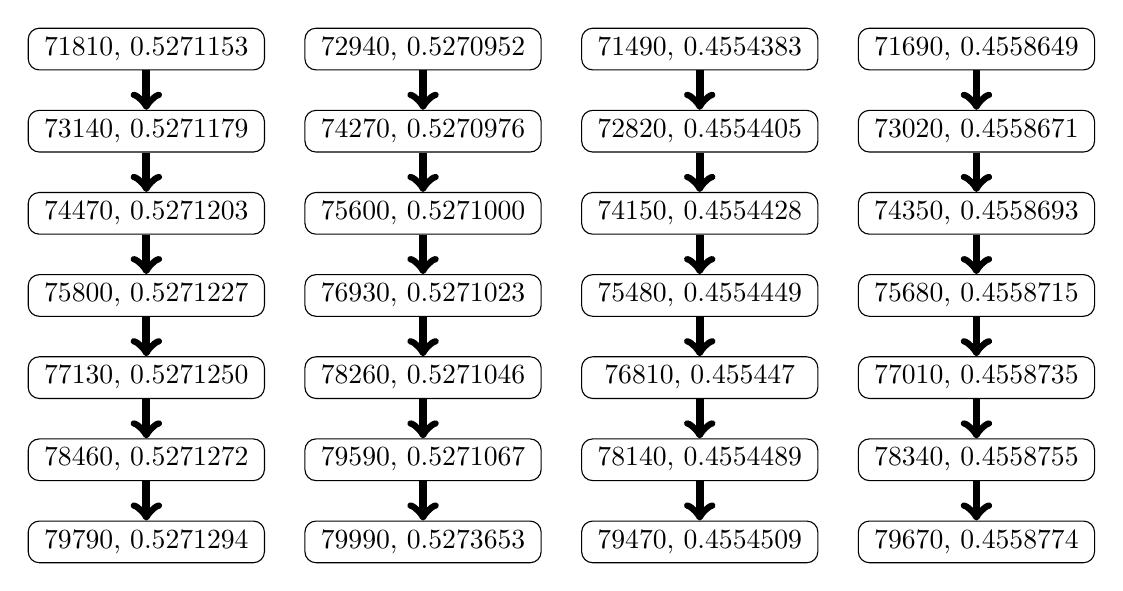
\begin{tikzpicture}[node distance=0.5cm, every node/.style={draw, align=center, minimum width=3cm, rounded corners}]
    
        % Define nodes (keeping only two smallest and two largest sets)
        \node (A1) {71810, 0.5271153};
        \node (A2) [right=of A1] {72940, 0.5270952};
        \node (A3) [right=of A2] {71490, 0.4554383};
        \node (A4) [right=of A3] {71690, 0.4558649};

        \node (B1) [below=of A1] {73140, 0.5271179};
        \node (B2) [below=of A2] {74270, 0.5270976};
        \node (B3) [below=of A3] {72820, 0.4554405};
        \node (B4) [below=of A4] {73020, 0.4558671};

        \node (C1) [below=of B1] {74470, 0.5271203};
        \node (C2) [below=of B2] {75600, 0.5271000};
        \node (C3) [below=of B3] {74150, 0.4554428};
        \node (C4) [below=of B4] {74350, 0.4558693};

        \node (D1) [below=of C1] {75800, 0.5271227};
        \node (D2) [below=of C2] {76930, 0.5271023};
        \node (D3) [below=of C3] {75480, 0.4554449};
        \node (D4) [below=of C4] {75680, 0.4558715};

        \node (E1) [below=of D1] {77130, 0.5271250};
        \node (E2) [below=of D2] {78260, 0.5271046};
        \node (E3) [below=of D3] {76810, 0.455447};
        \node (E4) [below=of D4] {77010, 0.4558735};

        \node (F1) [below=of E1] {78460, 0.5271272};
        \node (F2) [below=of E2] {79590, 0.5271067};
        \node (F3) [below=of E3] {78140, 0.4554489};
        \node (F4) [below=of E4] {78340, 0.4558755};

        \node (G1) [below=of F1] {79790, 0.5271294};
        \node (G2) [below=of F2] {79990, 0.5273653};
        \node (G3) [below=of F3] {79470, 0.4554509};
        \node (G4) [below=of F4] {79670, 0.4558774};
    
        % Draw thicker downward arrows
        \foreach \X/\Y in {A1/B1, B1/C1, C1/D1, D1/E1, E1/F1, F1/G1} {
            \draw[->, line width=1mm] (\X) -- (\Y);
        }
    
        \foreach \X/\Y in {A2/B2, B2/C2, C2/D2, D2/E2, E2/F2, F2/G2} {
            \draw[->, line width=1mm] (\X) -- (\Y);
        }
    
        \foreach \X/\Y in {A3/B3, B3/C3, C3/D3, D3/E3, E3/F3, F3/G3} {
            \draw[->, line width=1mm] (\X) -- (\Y);
        }
    
        \foreach \X/\Y in {A4/B4, B4/C4, C4/D4, D4/E4, E4/F4, F4/G4} {
            \draw[->, line width=1mm] (\X) -- (\Y);
        }

    \end{tikzpicture}
    \caption{Logarithmic convexity of last 7 consecutive 13-term summation ratios}
    \label{boundary_log_convexity}
\end{figure}

What is also evident when examining the upper two and lower two families of data points in Figure \ref{boundary_log_convexity} is that the logarithmic convexity of the sequence continues to manifest itself.  The ratios (per family) are still increasing even with integer denominators in the $2^{126,800} \simeq 10^{38,190}$ range at $n=80000$.  The impedance of term growth is constantly increasing in strength since consecutive term summation ratios can never decrease per family.

Figure \ref{boundary_log_convexity} shows last 7 values where $n<80,000$ for the two smallest and two largest ratios.  The first number is n and the second value is consecutive ratio.  As you go down a column you continue to see the ratio increase.

What this means is that 13-term summations will persist as the prevalent mode in the sequence.  This will be tempered with 12-term summations so not to span beyond the next $2^{-k}$ boundary.  There will continue to be the occasional 14-term summation balanced on both sides by 12-term summations, but term growth plateaus here.
%Term growth in addition to what was observed to cover the subsequent $2^{-k}$ brackets is possible beyond the flattened portions ($n > 80000$) shown in Figure \ref{12_term_coverage} and Figure \ref{13_term_coverage}.  However in order place Proposition \ref{cumulative_gt_binom_prop} in jeopardy the term growth rate needs to be linear in $k$.
%
%The rate of term growth cannot increase though due to the monotonically increasing consecutive ratio growth caused by the logarithmic convexity of \OEIS{A186009} and therefore it can never catch up to the linear growth rate of the binomial.

%\pagebreak
Thus it is always possible to group incremental novel convergence terms such that $N(n) > 2^{-k}; \forall k, k \in \setNo$ such that $n \le \binom{k}{k-2}$.  And since $C(n)$ is composed of the sum of $N(n)$ components, it therefore also exceeds $C(n) > \frac{2^{k-1}-1}{2^{k-1}}$.

Thus, is it shown that Proposition \ref{cumulative_gt_binom_prop} is true and we can assert:

\begin{equation}
\label{cumulative_gt_binom}
	C\binom{k}{k-2} > \frac{2^{k-1}-1}{2^{k-1}}; \forall k, k \in \setNo
\end{equation} 

What this is stating is that it is the cumulative portion $C(n)$ of the positive integer space which is guaranteed to converge (have a finite $\sigma(x)$ stopping time) for $n = \binom{k}{k-2}$ is strictly greater than the expression on the right hand side of \ref{cumulative_gt_binom}.


\pagebreak
\section{Conclusion}

We begin the conclusion with a simple relation:
\begin{equation}
\label{binomial_limit}
\lim_{k \to \infty} \frac{2^{k-1}-1}{2^{k-1}} = 1
\end{equation}

Also note that the first derivative of the logarithm of $\binom{k}{k-2}$ is concave:

\begin{equation}
\label{pascal_concave}
\frac{d}{dk} ln\binom{k}{k-2} = \frac{1-2k}{k-k^2}
\end{equation}

The logarithmic concavity is also evident through a visual inspection of Figure \ref{cn_bk}.  We now proceed through the final steps of the proof.

\begin{theorem}
    \label{cumulative_bracketing}
    It is possible to create an associative collection of residual classes fractions derived from the series \OEIS{A186009} which is $\ge \frac{2^{k-1}-1}{2^{k-1}}; \forall n, n \in \setN$
\end{theorem}

\begin{proof}
The series \OEIS{A186009} has been shown to be logarithmically convex by Theorem \ref{A186009_convex} whereas the $k-2$ diagonal of Pascal's Triangle is logarithmically concave by Equation \ref{pascal_concave}.  The convexity of \OEIS{A186009} ensures that the series will continue to grow exponentially and that the average compound factor will grow with increasing $n$. And, finally, by Equation \ref{cumulative_gt_binom}, we know that it is always possible to group residue fraction contributions which are greater than or equal to $\ge \frac{2^{k-1}-1}{2^{k-1}}$.
\end{proof}

\begin{theorem}
    \label{cumulative_limit_eq_1}
    The cumulative convergence, $C(n) = 1$ as $n$ goes to infinity.
\end{theorem}

% Theoretical relation we are trying to prove
\begin{proof}
	If we set $n = \binom{k}{k-2}$ then by Theorem \ref{cumulative_bracketing}:
%    \label{cumulative_convergence_theorem}
    \begin{equation}
      \frac{2^{k-1}-1}{2^{k-1}} \le \sum_{n=0}^{n} C(n) \le 1
    \end{equation} 
    By Equation \ref{cumulative_bracketing}, the left hand side converges to 1 as $k$ goes to $\infty$ which then by the Squeeze Theorem ensures
    \begin{equation}
		\lim_{n \to \infty} \sum_{n=0}^{n} C(n) = 1
    \end{equation} 
\end{proof}

Theorem \ref{cumulative_limit_eq_1} means that the proposition \ref{cumulative_convergence_prop} is in fact true.  By Squeeze Theorem, the series converges to unity and all positive integers eventually converge to a smaller value over a convergent subsequence.

Which leads to the final conclusion.
\begin{theorem}
    \label{Collatz_conjecture}
    The Collatz Conjecture is true.
\end{theorem}
\begin{proof}
By Theorem \ref{cumulative_limit_eq_1} all positive integers eventually converge to a smaller value.  Then by chaining together consecutive convergent subsequences of residue classes one creates a sequence which culminates in the terminal 4\Rarr2\Rarr1\Rarr4 cycle, passing through 1 \emph{before} cycling back to 4 in accord with the Collatz Conjecture.
\end{proof}


\newpage
\begin{thebibliography}{unsrt}

\bibitem{OEIS_A186009}
N. J. A. Sloane, \emph{OEIS A186009: Sequence A100982 with 1 prepended.}, 2011.  
Available at: \url{https://oeis.org/A186009}

\bibitem{OEIS_A047749}
N. J. A. Sloane, \emph{OEIS A047749: even: $\frac{1}{2m+1}\binom{3m}{m}$, odd: $\frac{1}{2m+1}\binom{3m+1}{m+1}$}, 2008.  
Available at: \url{https://oeis.org/A186009}

\bibitem{Winkler_Stopping}
Mike Winkler, \emph{The algorithmic structure of the finite stopping time behavior of the 3x + 1 function}, Nov. 2017.  
Available at: \url{http://arxiv.org/pdf/1709.03385v3.pdf}

\bibitem{Associative_Property}
Mattias Flygare, \emph{Some Properties of Infinite Series}, Master’s thesis, Karlstad University, 2012.  
Available at: \url{https://www.diva-portal.org/smash/get/diva2:535147/FULLTEXT01.pdf}

\bibitem{andrews1985special}
George E. Andrews, Richard Askey, and Ranjan Roy, \emph{Special Functions}, Cambridge University Press, 1985.

\bibitem{OEIS_A100892}
N. J. A. Sloane, \emph{OEIS A100982: Length of Collatz dropping time patterns}, 2005.  
Available at: \url{https://oeis.org/A100982}

\bibitem{OEIS_A020914}
N. J. A. Sloane, \emph{OEIS A020914: Allowable values of the dropping time in the Collatz problem}, 2006.  
Available at: \url{https://oeis.org/A020914}

\end{thebibliography}



\newpage
\appendix
\section{Finding Novel Residue Classes}
\label{novel_appendix}

This section describes how to find convergent subsequences of a given length in such a way as to exclude any convergent subsequences of a shorter length.  In other words, this method ensures that residue classes with smaller stopping times are filtered out leaving only the novel ones which emerged solely as a consequence of introducing a longer subsequence.

The method begins by creating a table with column headings which follow \OEIS{A020914} since this sequence indicates when new residue classes emerge as a result of increasing subsequence length.  To find novel convergent subsequences, the horizontal sum at every point in the row is strictly less than the column heading which will be a value taken from \OEIS{A020914}.  The exception is the last column where the horizontal sum needs to sum up to \emph{exactly} the value in that column.

The final column of a row solution must match because it is the total powers of 2 in the subsequence which is $A020914(n)$.  For $n \ge 1$ the minimum value in every column is 1 because all odd integers experience \emph{at least} one $3x+1$ expansion.  The lone exception to this rule is the first column $A020914(n=0)$ case which corresponds to the even integers.

For the first solution, representing the even numbers, $n=0$ and there is a single down-leg using one division factor of 2 to reach a smaller positive integer.  Even numbers are the only ones that have no up-legs.  Odd numbers have \emph{at least} one.

All odd numbers begin with 0 in the $n=0$ column for the number of factors of two in the initial down-leg.  Each immediately experiences a single $3x+1$ expansion as it moves along its subsequence, so each column from then on has a minimum value of 1 factor of 2 following the expansion.

The rules for finding novel convergent subsequences are:

\begin{enumerate}
\item The horizontal sum of all numbers in a row equals $A020914(k)$, where $k$ is the number of up-legs in the subsequence, i.e. $\sum_{i=0}^{k}$ row$(i) = A020914(k)$.
\item The horizontal sum at every point in the row before $A020914(k)$, where $k$ is the number of up-legs in the subsequence, less than $A020914(i)$ where $0 \le i < k$, i.e. $\forall i; i<k; i \in \setNo; \sum_{n=0}^{i} $row$(i) < A020914(i)$.
\item Continue to search for solutions which satisfy the previous rules until all valid combinations are found.
\end{enumerate}

\pagebreak
Rule 2 filters out shorter stopping time residue classes.  By matching the horizontal sum of the total number of factors of two for the last column, but remaining strictly less for previous columns, shorter stopping time solutions are suppressed.

There are a number of ways to execute the algorithm however the approach taken in Figure \ref{subsequences} below defines a search process for odd numbers ($k \ge 1$) leading with a 0, followed by 1's in all columns prior to the $k^{th}$ column and in the last column placing the integer $A020914(k) - (k-1)$, which brings the horizontal sum total to $A020914(k)$.

For example, for $n=4, A020914(4)=7$.  Thus the starting point is 0\Rarr 1\Rarr 1\Rarr 1\Rarr 4 and the horizontal sum is 7 in the last column.  In Figure \ref{subsequences}, the horizontal sum of the entries up to column $n=i$ is given by $H(i) = \sum_{0}^i $row($i$), where $i$ spans the row entries up to the $n=i$ column.  In Figure \ref{subsequences}, $A(i)$ is short-hand for $A020914(i)$.


% Flowchart shows how to find all the convergent subsequences of a given length, k > 0
\begin{figure}[ht]				% the [ht] places here or top of page
\caption{Finding convergent subsequences of length $k; k \in \setN$}
\label{subsequences}

\begin{center}
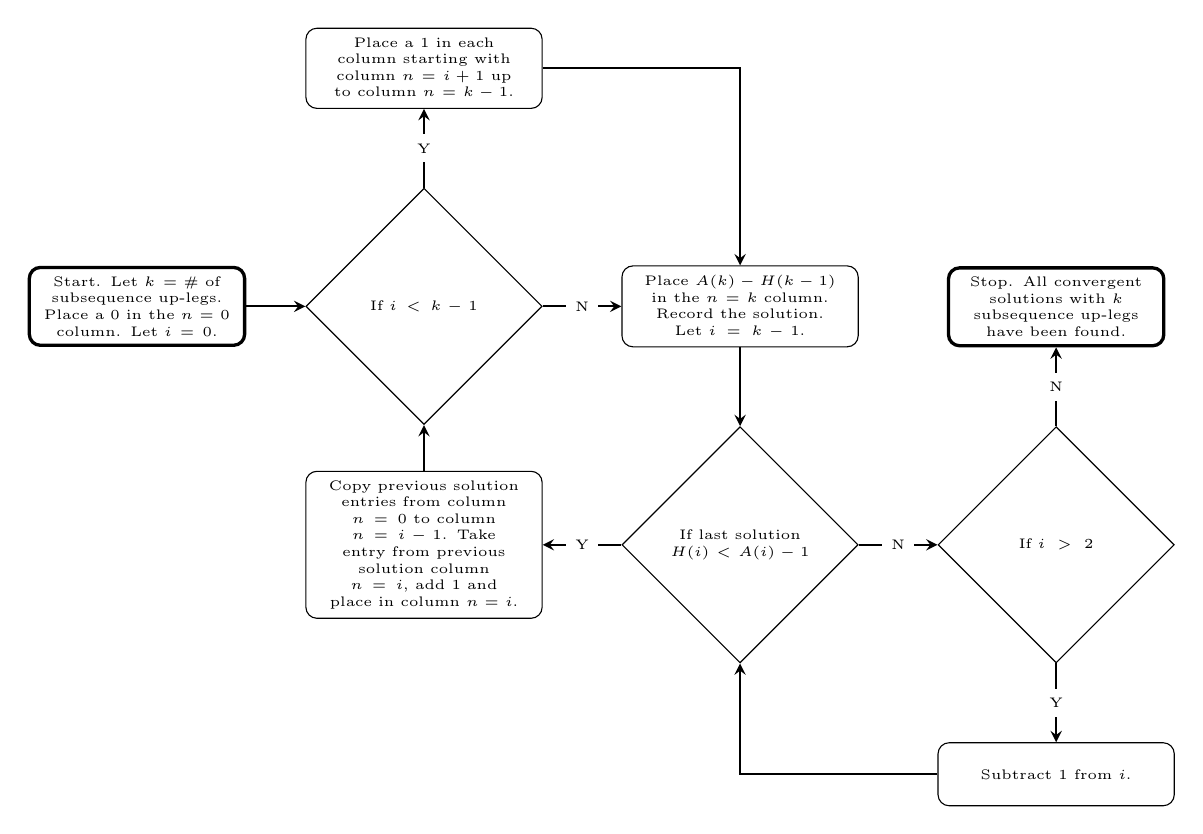
\begin{tikzpicture}[node distance=0.75cm, font = \tiny] % Default node spacing and font size

% Place the nodes on the flowchart
\node(start)        [startstop]                           {Start. Let $k = $ \# of subsequence up-legs. Place a $0$ in the $n=0$ column.  Let $i=0$.};
\node(i_lt_k-1)     [decision,  right=of start]           {If $i < k-1$};
\node(carry_ones)   [action,    above=1.0cm of i_lt_k-1]  {Place a 1 in each column starting with column $n=i+1$ up to column $n=k-1$.};
\node(remainder)    [action,    right=1.0cm of i_lt_k-1]  {Place $A(k)-H(k-1)$ in the $n=k$ column. Record the solution. Let $i = k-1$. };
\node(i_lt_A)       [decision,  below=1.0cm of remainder] {If last solution $H(i)<A(i)-1$};
\node(copy_inc)     [action,    left=1.0cm of i_lt_A]     {Copy previous solution entries from column $n=0$ to column $n=i-1$. Take entry from previous solution column $n=i$, add 1 and place in column $n=i$.};
\node(i_gt_2)       [decision,  right=1.0cm of i_lt_A]    {If $i>2$};
\node(decrement_i)  [action,    below=1.0cm of i_gt_2]    {Subtract 1 from $i$.};
\node(stop)         [startstop, above=1.0cm of i_gt_2]    {Stop. All convergent solutions with  $k$ subsequence up-legs have been found.};

% Connect the nodes with arrows
\draw [arrow] (start)        --                       (i_lt_k-1);
\draw [arrow] (i_lt_k-1)     -- node[fill=white,] {Y} (carry_ones);
\draw [arrow] (i_lt_k-1)     -- node[fill=white,] {N} (remainder);
\draw [arrow] (carry_ones)   -|                       (remainder);
\draw [arrow] (remainder)    --                       (i_lt_A);
\draw [arrow] (i_lt_A)       -- node[fill=white,] {Y} (copy_inc);
\draw [arrow] (i_lt_A)       -- node[fill=white,] {N} (i_gt_2);
\draw [arrow] (copy_inc)     --                       (i_lt_k-1);
\draw [arrow] (i_gt_2)       -- node[fill=white,] {Y} (decrement_i);
\draw [arrow] (decrement_i)  -|                       (i_lt_A);
\draw [arrow] (i_gt_2)       -- node[fill=white,] {N} (stop);

\end{tikzpicture}
\end{center}
\end{figure}

%\newpage
%\appendix
%\renewcommand{\thesection}{Appendix \Alph{section}:} % Prefix "Appendix" to section labels
%\section{Auxiliary Numerical Graphics}
%\label{novel_appendix}

\newpage
\section{Auxiliary Numerical Graphics}
\label{auxiliary_graphics}

The following shows the 10-term and 11-term consecutive ratios.  Note that these both exceed $\frac{1}{2}$ however they are smaller than what is required to cover the subsequent $\frac{1}{2^{n}}$ bracket for $n>100$ and $n>500$ respectively.

\begin{figure}[h]				% the [ht] places here or top of page
    \centering
    % LaTeX cannot follow symbolic links.  Need true directories and files.
    \includegraphics[width=\linewidth]{./figures/10_Term_Group_Ratios.pdf}
    \caption{Ratio of 10-term sum divided by prior 10-term sum}
    \label{10-term-group-ratios}
\end{figure}

\begin{figure}[H]				% the [H] forces placement here (float package)
    \centering
    % LaTeX cannot follow symbolic links.  Need true directories and files.
    \includegraphics[width=\linewidth]{./figures/11_Term_Group_Ratios.pdf}
    \caption{Ratio of 11-term sum divided by prior 11-term sum}
    \label{11-term-group-ratios}
\end{figure}

The following shows the 14-term and 15-term consecutive ratios.  Note that these both fall short of $\frac{1}{2}$ however they are larger than is required to cover the subsequent $\frac{1}{2^{n}}$ bracket.  14-terms summations are observed to happen but 15-term summations are not possible, and therefore 14-term summation serves as the upper limit.

\begin{figure}[ht]				% the [ht] places here or top of page
    \centering
    % LaTeX cannot follow symbolic links.  Need true directories and files.
    \includegraphics[width=\linewidth]{./figures/14_Term_Group_Ratios.pdf}
    \caption{Ratio of 14-term sum divided by prior 14-term sum}
    \label{14-term-group-ratios}
\end{figure}

\begin{figure}[H]				% the [H] forces placement here (float package)
    \centering
    % LaTeX cannot follow symbolic links.  Need true directories and files.
    \includegraphics[width=\linewidth]{./figures/15_Term_Group_Ratios.pdf}
    \caption{Ratio of 15-term sum divided by prior 15-term sum}
    \label{15-term-group-ratios}
\end{figure}

\end{document}  

